%% main.tex -- MDPI Applied Sciences manuscript, revision v6 (fifth review reflected; rev10 experiments, kernel v3.3).
%% Overleaf: paste into the official MDPI template project; the Definitions/ folder with
%% mdpi.cls, mdpi.bst and logos is supplied by the template.
%% Companion files: refs.bib, fig_threat.tex, fig_overview.tex, fig_kernel.tex, figs/fig_scores.pdf, figs/fig_holdout.pdf, figs/fig_roc.pdf, figs/fig_factors.pdf, figs/fig_witness.pdf.
\documentclass[applsci,article,submit,pdftex,moreauthors]{Definitions/mdpi}

%--------------------------------------------------------------------- packages
\usepackage{tikz}
\usetikzlibrary{positioning,arrows.meta,calc,fit,decorations.pathreplacing,shapes.geometric}
\usepackage{booktabs}
\usepackage{multirow}
\usepackage{amsmath}
\usepackage{algorithm}
\usepackage{algorithmic}
\newcommand{\holdoutconf}{240}\newcommand{\attrconf}{158}
% left-aligned, non-hyphenating table columns (Y: flexible, Q{w}: fixed width)
\newcolumntype{Y}{>{\raggedright\arraybackslash\hyphenpenalty=10000\exhyphenpenalty=10000}X}
\newcolumntype{Q}[1]{>{\raggedright\arraybackslash\hyphenpenalty=10000\exhyphenpenalty=10000}p{#1}}
\renewcommand{\topfraction}{0.92}\renewcommand{\bottomfraction}{0.6}\renewcommand{\textfraction}{0.05}\renewcommand{\floatpagefraction}{0.85}
\newcolumntype{Z}{>{\raggedright\arraybackslash\hyphenpenalty=10000\exhyphenpenalty=10000}l}

%--------------------------------------------------------------------- front matter
\firstpage{1}
\makeatletter
\setcounter{page}{\@firstpage}
\makeatother
\pubvolume{16}
\issuenum{1}
\articlenumber{0}
\pubyear{2026}
\copyrightyear{2026}
\datereceived{ }
\daterevised{ }
\dateaccepted{ }
\datepublished{ }
\hreflink{https://doi.org/}

\Title{Spatio-Temporal Provenance Guard: Detecting Privilege Escalation Attacks that Exploit Spatio-Temporal Data Loss in Multi-Agent MCP Environments}
\TitleCitation{Spatio-Temporal Provenance Guard: Detecting Privilege Escalation Attacks that Exploit Spatio-Temporal Data Loss in Multi-Agent MCP Environments}

% Affiliation, e-mail and ORCID are to be completed by the authors.
\newcommand{\orcidauthorA}{0000-0000-0000-000X}
\Author{Deuk-Hun Kim $^{1}$\orcidA{} and Jin Kwak $^{2,*}$}
\AuthorNames{Deuk-Hun Kim and Jin Kwak}
\AuthorCitation{Kim, D.-H.; Kwak, J.}
\address{%
$^{1}$ \quad Affiliation 1; e-mail\\
$^{2}$ \quad Affiliation 2; e-mail}
\corres{Correspondence: e-mail}

\abstract{MCP (Model Context Protocol) agents reuse shared records across sessions, and the provenance of a record (source, writer, trust, privilege) is normally dropped at storage boundaries; because records are dispersed over hiding locations and over sessions, we call this spatio-temporal data loss. An adversary controlling only an ingestion path can spread an outbound-transfer directive over individually incomplete records that a high-privilege agent later assembles. We present STPG (Spatio-Temporal Provenance Guard), a gateway defense that persists connector provenance on write, reassembles records by lineage on read, and authorizes routing calls through a destination-conditioned witness verified against a deterministic support path. On a Google Cloud testbed with 918 Gemini-driven traces, STPG blocked all 648 attacks and passed all 71 approved external transfers issued, whereas a conservative provenance gate blocked all 71 and an attribution judge 16. On 180 challenge traces and 240 counterfactual calls, STPG matched every specified decision and passed 84 of 108 business-approved calls under its provenance and hop policies; structural verification rejected 116 of 330 positive lineage-level witness verdicts, and actual-call conformance was 175 of 176. In an ablation, the untrusted-directive branch leaves default-deny decisions unchanged but prevents all attacks under an allow-on-empty default.}

\keyword{multi-agent systems; Model Context Protocol; data provenance; privilege escalation; AI security}

\begin{document}

%=====================================================================
\section{Introduction}
\label{sec:intro}

LLM (Large Language Model) agents have moved from a single agent that calls tools to systems in which several agents with separate roles cooperate \cite{wang2024agents,xi2025rise}. MCP (Model Context Protocol) standardizes how an agent discovers and invokes tools, reads data sources, and exchanges state \cite{mcpspec}; MCP-based multi-agent deployments are proposed for security operations \cite{mcpsoc2026} and combined with zero-trust monitoring in multi-cloud operations \cite{mcloudzt2026}. Interconnection enlarges the attack surface: inter-agent messages, shared stores, delegated privileges, and untrusted content that enters through ingestion paths become points of entry, and indirect prompt injection \cite{greshake2023}, the confused-deputy problem \cite{hardy1988}, and privilege escalation are among the core threats to agent systems \cite{agentsurvey2026,yao2024survey}.

This paper studies one property of such systems as an attack enabler: data accumulates across storage boundaries and sessions, and the metadata that would tell a later reader where a record came from is normally not stored with it. We call this loss of provenance at storage and session boundaries spatio-temporal data loss; the data itself survives, its provenance does not. The loss has a spatial dimension, the dispersion of records over hiding locations and stores (a log message, a ticket body, an API (Application Programming Interface) description field, each read through a different path), and a temporal dimension, the dispersion over sessions that have ended by the time the record is read. An adversary who controls only an ingestion path can exploit both without writing a complete instruction anywhere: the parts of an outbound-transfer directive are placed in several records that each read as an operational note. When a high-privilege agent later reads the records of a domain into one context, the directive emerges and the agent forwards data to an external destination under its own privilege.

Two questions follow for a defense. The first is whether such an induced transfer can be stopped; in the configurations we evaluate, a gate that keeps provenance across the storage boundary and refuses an external transfer unless a trusted directive authorizes it does so. The second is whether such a gate can be deployed on a path that legitimately reads untrusted data: operations agents read intake notes, vendor advisories, and imported registries as a matter of course, and operators issue approved external transfers such as a standing rule that forwards a weekly report to a partner. A gate that treats untrusted influence as sufficient reason to block destroys this work; a gate that treats a trusted record naming the destination as sufficient reason to pass can be led astray by a trusted registry entry that merely mentions the destination, or by a trusted rule that names it only to prohibit it. The defense therefore has to answer, at the moment of the call, which records formed the directive behind it, whether that directive targets this destination, and whether it was authorized: the distinction between provenance and authorization that AuthGraph draws for single executions \cite{wang2026authgraph}, carried across the storage boundary and conditioned on the destination.

We propose STPG (Spatio-Temporal Provenance Guard), a defense inserted into the MCP gateway. PPT (Persistent Provenance Tagging) attaches a provenance sidecar to every record at write time, keyed by the authenticated source connector, so that lineage survives both boundaries. TSA (Temporal Shard Assembly) regroups, at read time, the records that share a lineage regardless of location and session, reassembles them, and scores whether the assembled text forms an external-transfer directive. PDG (Privilege-Delta Gate) binds the destination of the actual call to the lineages that name it, directly or through registry references, asks a destination-conditioned witness whether a binding lineage targets that destination, verifies the verdict against a deterministic support path, and applies one kernel: pass on a trusted directive, block on an untrusted one, block by default. Absence of detection is not treated as authorization.

The contributions are: (i) a threat model of privilege escalation through spatio-temporal data loss with four conditions, each mapped to the defense limitation it exploits; (ii) STPG specified as one decision kernel, with a decision table and an algorithm covering binding, reference resolution with ambiguity and hop limits, an endpoint pre-check, destination-conditioned witnessing with support-path verification, and missing and empty evidence, and every comparison condition specified as an evidence adapter on that kernel; (iii) an evaluation on a cloud testbed driven by real LLM agents against eight comparison conditions, two of them ablations of STPG, with hard benign negatives that mirror the attack's surface form, a metadata probe whose limits we state, a policy challenge set of fifteen structures evaluated counterfactually on every listed destination, raw counts with cluster-aware statistics over both template classes, and measured cost per condition.

The remainder of this paper is organized as follows. Section~\ref{sec:related} reviews related work. Section~\ref{sec:problem} analyzes the problem and the limitations of existing defenses. Section~\ref{sec:improve} derives the improvements and hypotheses. Section~\ref{sec:method} presents the proposed method, STPG. Section~\ref{sec:exp} describes the experimental setup. Section~\ref{sec:results} reports the experimental results. Finally, Section~\ref{sec:conclusion} concludes the paper.

%=====================================================================
\section{Related Work}
\label{sec:related}

\subsection{Threats to LLM Agents and Multi-Agent MCP Systems}
Surveys of LLM-agent security list indirect prompt injection, privilege escalation, and confused-deputy behavior as recurring threats \cite{agentsurvey2026,yao2024survey}. Indirect prompt injection, in which an instruction hides in content the agent retrieves, was demonstrated against real LLM-integrated applications \cite{greshake2023}, and InjecAgent benchmarks it for tool-integrated agents with direct-harm and data-stealing cases \cite{zhan2024injecagent}; the confused deputy predates LLMs \cite{hardy1988}. These threat models assume that the injected instruction is complete within the retrieved content. Multi-agent MCP frameworks for operations, such as the security-operations design of Sim\~oes et al.~\cite{mcpsoc2026}, concentrate on authentication, authorization, and auditing of agent-to-tool traffic.

\subsection{Fragment Assembly and Cross-Session Threats}
\label{sec:rel-assembly}
Liu et al.\ show that summarization-based prompt compression relinks fragments that are each benign in the source into a complete malicious instruction in the summary \cite{liu2026relink}; their KBRA (Keyed Binding Reassembly Audit) extracts predicate--role--value bindings from source and action, uses provenance-aware channel information with exact or semantic matching, and requires that the bindings behind an action be supported by a single source segment. Relink is the closest mechanism to our assembly condition, but its fragments live in one carrier document inside one context and its boundary is compression, whereas ours are records written by other principals in earlier sessions and the boundary is storage; KBRA's unit is a source segment, STPG's is a lineage keyed by the authenticated source connector or by an individual trusted write, with reference chains that may cross lineages.

CSTM-Bench provides cross-session scenarios that accumulate, compose, launder, or inject on the reader, with per-reader role policies, judged by a reader LLM over the session log \cite{azarafrooz2026cstm}; XSPI (Cross-Session Stored Prompt Injection) is evaluated in a stateful sandbox with persistent memory and executable tools over 486 cases, including payload splitting across agents \cite{xie2026xspi}. Neither models writer identity and privilege as a stored attribute of records, approved external transfers as a benign class, or a sink decision that separates an induced transfer from an authorized one (Section~\ref{sec:data}).

\subsection{Provenance and Authorization in Agent Actions}
\label{sec:rel-prov}
\paragraph{Provenance within one execution}
CaMeL attaches capabilities, which record provenance and permitted readers, to every value inside a custom interpreter and checks policies before each tool call \cite{debenedetti2025camel}. AuthGraph separates an injected reasoning graph from an authorization graph built from the user's prompt and checks the allowed origin of each security-critical parameter \cite{wang2026authgraph}. PFI (Prompt Flow Integrity) separates trusted and untrusted agents, checks the source trust of tool outputs, treats unknown sources as untrusted, and keeps an explicit user-approval path across the trust boundary \cite{kim2025pfi}. CapChain combines capability tokens with a signed provenance log that gates state merges in multi-agent workflows \cite{capchain2026}. In all four, provenance lives within one plan, one execution, one tool call, or one state store, and authorization derives from a user prompt, a capability policy, or a user approval. STPG differs in two respects: the producer provenance is persisted with the record, attributed to an authenticated principal with a trust level, and re-read in a later session by a different agent for which no per-request user prompt exists; our ephemeral-taint condition reproduces only a taint that is not persisted at the storage boundary, not PFI or CaMeL.

\paragraph{Persistent provenance with action authorization}
Three recent preprints combine persistence and authorization, which is the conjunction that STPG relies on, and we cite them as preprints because the comparison would be incomplete without them.
\begin{itemize}
\item MemLineage keeps a signed append-only log per principal and a derivation graph of memory entries; an entry inherits the least trusted of its strongly connected parents, and a sensitive-action gate names, per governed parameter, the source classes allowed to authorize it. It reports zero attack success with a legitimate-dispatch rate of 1.00 on a deterministic harness \cite{ouyang2026memlineage}.
\item PPMF proposes platform-maintained provenance with source and confirmation labels and a deterministic support binding that matches an action's canonical target to memory entries, resolves aliases only through a platform mapping, returns all candidates when ambiguous, and authorizes at the minimum trust of the support; it reports zero attack success with benign success 1.000 under intact provenance \cite{xu2026ppmf}.
\item Sleeper Channels tags artifacts by channel, principal, and device, closes memory operations over their causal sources, and allows an action when its causal set is entirely trusted or an owner grant bound to the action digest exists; its evaluation is preregistered as follow-on work \cite{maloyan2026sleeper}.
\end{itemize}
Two of their mechanisms are close to ours: PPMF's alias resolution and all-candidates rule correspond to STPG's reference resolution and ambiguity rule, and MemLineage's per-parameter authority to STPG's destination-level scope. The differences we claim are narrower than a new principle. First, STPG groups records that other principals write to a shared store by the authenticated source connector, so that records dispersed over locations and sessions are regrouped as one lineage; none of the three evaluates this grouping. Second, STPG's authorization evidence is a directive found in the stored records themselves, such as an operator's standing rule, that must be witnessed to target the destination of the actual call, with mention, mapping, and prohibition in the same text distinguished from instruction, and verified against a deterministic support path. Third, the evaluation covers mixed trusted and untrusted directives in one context under both empty defaults, with the untrusted branch isolated by ablation.

\paragraph{Other related areas}
Classical information-flow control \cite{denning1976,sabelfeld2003} and the provenance literature \cite{provsurvey2023,li2021provgraph} provide the lattice and the tracking machinery; they do not define which records formed an LLM agent's directive or whether it was authorized for the destination it reached. Spotlight-Guard \cite{spotlight2026} and anomaly-detection agents for logs \cite{logresp2025} inspect content or behavior within a request and are complementary.

\paragraph{Summary of the gap}
Table~\ref{tab:related} summarizes the comparison. In the table, S denotes source trust and A action authorization with its basis (for KBRA, A denotes binding support rather than principal- or task-level authority); Persist.\ means that provenance survives storage and sessions, and Legit.\ ext.\ that approved external actions are evaluated as a benign class. The gap is the conjunction of persistence across both boundaries with principal attribution, a judgment unit defined by source lineage, and a sink decision that binds the actual call to lineages and witnesses that a binding lineage targets the destination.

\begin{table}[!htb]
\caption{Closest related work along the dimensions of the threat.}
\label{tab:related}
\begin{adjustwidth}{-\extralength}{0cm}
\footnotesize
\centering
\begin{tabularx}{\fulllength}{Q{2.0cm}YYQ{2.1cm}Q{1.35cm}Q{1.15cm}Q{2.0cm}}
\toprule
\textbf{Work} & \textbf{Boundary; unit} & \textbf{Decision basis} & \textbf{Trust} & \textbf{Persist.} & \textbf{Legit. ext.} & \textbf{Assembly} \\
\midrule
Relink/KBRA \cite{liu2026relink} & compression; source segment & source-supported binding, channel provenance & S (channel); A (binding support) & no & yes & within a document \\
CSTM-Bench \cite{azarafrooz2026cstm} & sessions as transcripts; reader LLM & correlation vs.\ per-role policy & A (role policy) & no & partial & by the reader \\
XSPI \cite{xie2026xspi} & stored injection; stateful sandbox & guardrails, tool-call outcome & no & memory & no & no \\
CaMeL \cite{debenedetti2025camel} & one plan execution; values & capabilities vs.\ policy & S; A (capability policy) & no & yes & no \\
AuthGraph \cite{wang2026authgraph} & one execution; tool parameters & parameter origin vs.\ authorization graph & S; A (user prompt) & no & yes & no \\
PFI \cite{kim2025pfi} & tool call; agent/tool output & source trust check & S; A (user approval) & no & yes & no \\
CapChain \cite{capchain2026} & state merge; field & capability token & S & in-store & no & no \\
MemLineage \cite{ouyang2026memlineage} & agent memory; entry with derivation graph & least trusted strong parent; per-parameter source-class authority with repair & S (lineage); A (parameter source class) & yes (signed log) & yes & derivation graph, not directive \\
PPMF \cite{xu2026ppmf} & memory consolidation; entry & deterministic support binding to the canonical target, minimum trust, risk class & S; A (support trust vs.\ risk class) & yes (platform) & yes & no \\
Sleeper Channels \cite{maloyan2026sleeper} & time boundary; artifact with causal set & trusted causal set, or owner grant over the action digest (design) & S (channel, principal, device); A (owner grant) & yes & -- & no \\
\textbf{STPG (ours)} & storage and session; principal lineage & destination-witnessed, path-verified lineage trust & S; A (trusted directive targets $\delta$) & yes & yes & across locations and sessions \\
\bottomrule
\end{tabularx}
\end{adjustwidth}
\end{table}

%=====================================================================
\section{Analysis of Problem and Limitation}
\label{sec:problem}

\subsection{System Model}
\label{sec:system}
A multi-agent MCP environment consists of agents $a$ with a trust level $\tau(a)$ and a privilege level $\pi(a)$, an MCP gateway through which every write, read, and tool call passes, and a shared store of records. We use four trust levels, $\tau_{\mathrm{ext}}<\tau_{\mathrm{ingest}}<\tau_{\mathrm{ops}}<\tau_{\mathrm{sys}}$, and four privilege levels, read, write, API, and IAM (Identity and Access Management). An ingest agent with trust $\tau_{\mathrm{ingest}}$ and privilege write writes content that enters through an ingestion endpoint; such content is assigned source trust $\tau_{\mathrm{ext}}$ regardless of the writer. An operations agent with trust $\tau_{\mathrm{ops}}$ and privilege IAM periodically reads the accumulated records of a domain in one read and decides its next step: a status report or a routing action that names a destination. Destinations on an approved allow-list are internal; every other destination is external. Privilege separation is enforced by identity: the two agents run under separate service accounts, the gateway refuses a tool outside the caller's profile and labels each write with the identity and endpoint through which it arrived, and the ingest identity's call to the privileged routing tool is refused. Each session has a separate gateway session identifier; the agent carries no memory across sessions, and the store persists.

\subsection{Threat Model}
\label{sec:threat}
The adversary controls the external ingestion path only. It can insert records whose bodies read as operational notes, but it cannot change model weights, system prompts, the gateway, or the provenance sidecars, and it cannot forge the source identifier, which the gateway derives from the authenticated ingestion connector. Within this capability, the attack satisfies four conditions, which Figure~\ref{fig:threat} places on the two axes of the data loss.
\begin{enumerate}
\item \textbf{Individually incomplete:} No single one of the $k$ records names both an action and an external target. The term does not mean statistically indistinguishable; Section~\ref{sec:detection} reports that per-record scores separate the classes in part.
\item \textbf{Emergent on assembly:} With $m(\cdot)$ the degree to which a text functions as a complete instruction to route output externally, $m(s_i)$ is low for every record while $m(\{s_1,\dots,s_k\})$ is high, because the records resolve each other's references.
\item \textbf{Spatio-temporally dispersed:} Spatially, the records are spread over hiding locations and stores such as log messages, ticket bodies, and API description fields; temporally, over $d$ sessions, with ordinary records between them. A reader that groups by location, window, or session sees fragments; only grouping by source sees the set.
\item \textbf{Low trust to high privilege:} The records have source trust $\tau_{\mathrm{ext}}$ and the action is executed with privilege IAM. The privilege gap $g\in\{0,1\}$ states whether the writing identity also has lower privilege than the caller, $g=1$, which is a privilege escalation across identities, or is a high-privilege identity whose ingestion-path write is nevertheless untrusted, $g=0$, which is an induced unauthorized action; we report both and do not equate them.
\end{enumerate}
The same context may also contain an approved external transfer, a trusted operator's standing rule naming a partner, and the defense must separate the two external calls (Section~\ref{sec:holdout}). The attack depends on the loss of provenance, not on the detectability of any single record.

\begin{figure}[!htb]
\begin{adjustwidth}{-\extralength}{0cm}
\centering
\resizebox{0.98\fulllength}{!}{% fig_threat.tex -- spatio-temporal dispersion of the attack records and the loss of provenance (TikZ)
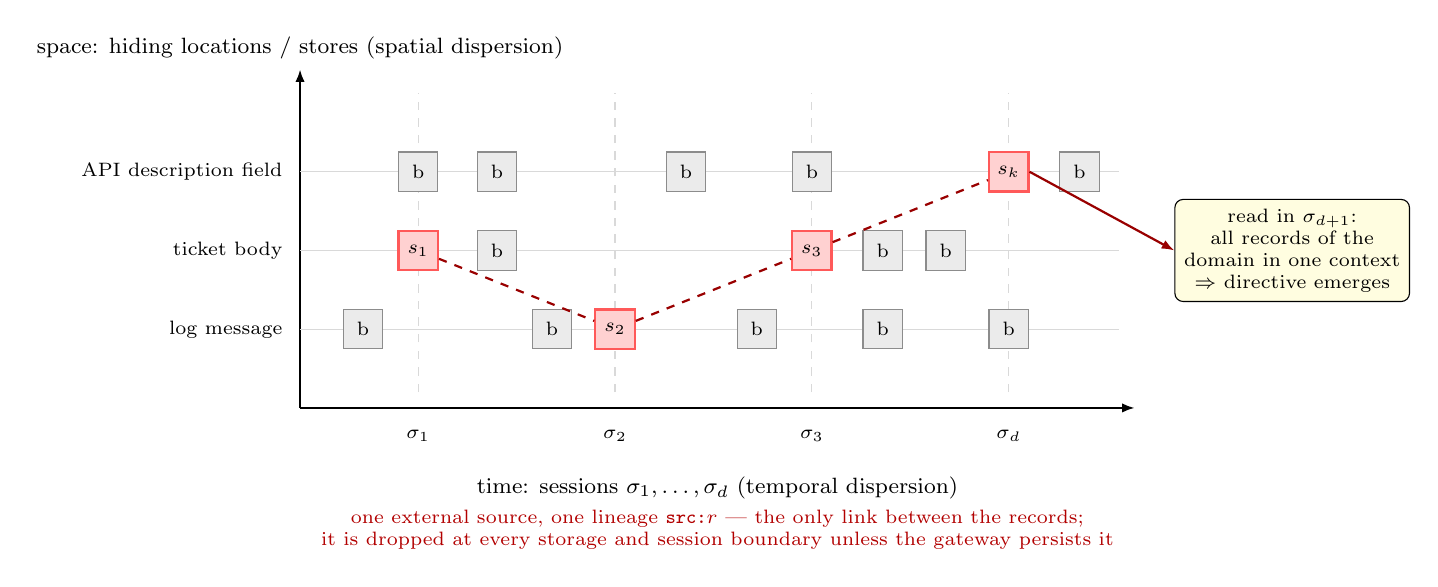
\begin{tikzpicture}[x=1cm,y=1cm,font=\footnotesize,>={Latex[length=1.6mm]},
  rec/.style={draw,minimum width=5mm,minimum height=5mm,inner sep=0pt,font=\scriptsize},
  shard/.style={rec,fill=red!18,draw=red!65,thick},
  benign/.style={rec,fill=black!8,draw=black!45},
  lab/.style={font=\scriptsize,text=black}]
% axes: x = sessions (time), y = locations/stores (space)
\draw[->,thick] (0,0)--(10.6,0); \node[font=\footnotesize,anchor=north] at (5.3,-0.75) {time: sessions $\sigma_1,\dots,\sigma_d$ (temporal dispersion)};
\draw[->,thick] (0,0)--(0,4.3) node[above,font=\footnotesize,align=center]{space: hiding locations / stores (spatial dispersion)};
\foreach \y/\n in {1/log message,2/ticket body,3/API description field}{\node[lab,anchor=east] at (-0.1,\y) {\n}; \draw[black!15] (0,\y)--(10.4,\y);}
\foreach \x/\s in {1.5/$\sigma_1$,4/$\sigma_2$,6.5/$\sigma_3$,9/$\sigma_d$}{\node[lab] at (\x,-0.35) {\s}; \draw[black!15,dashed] (\x,0.2)--(\x,4.0);}
% benign records
\foreach \x/\y in {0.8/1,2.5/2,1.5/3,3.2/1,4.9/3,5.8/1,7.4/2,6.5/3,8.2/2,9.9/3,9.0/1,2.5/3,7.4/1}{\node[benign] at (\x,\y) {b};}
% shards
\node[shard] (s1) at (1.5,2) {$s_1$}; \node[shard] (s2) at (4.0,1) {$s_2$}; \node[shard] (s3) at (6.5,2) {$s_3$}; \node[shard] (sk) at (9.0,3) {$s_k$};
\draw[red!60!black,dashed,thick] (s1)--(s2)--(s3)--(sk);
\node[lab,text=red!70!black,align=center] at (5.3,-1.55) {one external source, one lineage \texttt{src:}$r$ --- the only link between the records;\\it is dropped at every storage and session boundary unless the gateway persists it};
% assembly at read
\node[draw,fill=yellow!12,rounded corners=3pt,align=center,font=\scriptsize] (read) at (12.6,2.0) {read in $\sigma_{d+1}$:\\all records of the\\domain in one context\\$\Rightarrow$ directive emerges};
\draw[->,thick,red!60!black] (sk.east) -- (read.west);
\end{tikzpicture}
}
\end{adjustwidth}
\caption{Spatio-temporal dispersion of attack records (red) among ordinary records across sessions and hiding locations.}
\label{fig:threat}
\end{figure}

\subsection{Limitations of Existing Defenses}
\label{sec:limits}
Table~\ref{tab:limits} links each threat condition to the limitation it exploits, to the comparison condition that instantiates the limitation on the common kernel, and to the factor or challenge structure that stresses it. Three limitations concern what a defense can see and keep: a bounded window cannot contain a directive whose records lie outside it; provenance that lives inside one execution leaves the gate with no lineage once a record crosses the storage boundary (a property of non-persistence, not of PFI or CaMeL specifically); lexical signatures do not fire on lexically ordinary records. Three concern the decision: a gate that uses untrusted influence without attribution blocks every external call that any untrusted record touched; a gate that authorizes a call because a trusted record names its destination takes a mention for an authorization; a gate that checks the existence of a directive and the occurrence of the destination separately can be steered by a trusted rule that forwards to A while listing or prohibiting B. STPG is designed against the last three.

\begin{table}[!htb]
\caption{Threat conditions, the limitation each exploits, the comparison condition that instantiates it, and the stressing factor.}
\label{tab:limits}
\footnotesize
\begin{tabularx}{\textwidth}{Q{2.6cm}Q{3.2cm}Q{3.6cm}Y}
\toprule
\textbf{Threat condition} & \textbf{Limitation exploited} & \textbf{Condition on the kernel} & \textbf{Stressed by} \\
\midrule
emergent on assembly & bounded window; per-record scores & window scorer, unit inspection (detection only) & $k$, location \\
spatio-temporally dispersed & non-persistent provenance \cite{kim2025pfi,debenedetti2025camel} & ephemeral taint & $d$, location \\
individually incomplete & lexical signatures & unit inspection & $k$ \\
low trust to high privilege & no trust-coupled sink decision & undefended & $g$ \\
legitimate work reads untrusted data & influence without attribution & conservative gate; full-context attribution judge & approved transfers; mixed and bundle structures \\
trusted records mention the destination & mention taken as authorization & trusted-rule matching & cross-reference, trusted-mention, ambiguous-key structures \\
directive and destination in one trusted text & existence and occurrence checked separately & witness without support-path verification (analysis) & same-record, three-hop structures \\
\bottomrule
\end{tabularx}
\end{table}

%=====================================================================
\section{Derivation of Improvements}
\label{sec:improve}

The limitations in Table~\ref{tab:limits} lead to three design requirements and four hypotheses, each stated for the conditions evaluated rather than for defenses in general.

\paragraph{R1: bind provenance to data at write time and persist it across both boundaries}
In-execution taint cannot be reconstructed after the fact, so the source identity, the writer, and the writer's trust and privilege must be stored as a sidecar that any later reader in any session can resolve, whatever location the record was hidden in. Hypothesis H1: among the evaluated configurations, every condition that persists provenance and applies the default-deny kernel blocks the attack, and the ephemeral-taint configuration, which persists nothing and passes on empty evidence, does not. H1 compares configurations, not persistence alone: a gate with no provenance and the default-deny kernel would also block every external call, including the approved ones; persistence is what lets a gate pass approved work selectively.

\paragraph{R2: attribute the actual call to lineages, witness the destination, and decide on trust}
Because the directive exists only in the assembly, the unit of judgment is the set of records that share a source lineage. Because the same context can hold an approved and an induced transfer, the gate must bind the destination of the actual call to the lineages that name it, resolving registry references across lineages, and establish that a binding lineage targets that destination, not merely that a directive exists somewhere in it and the destination string occurs somewhere in it. A trusted record that mentions, lists, or prohibits the destination is not an authorization; absence of any directive is not one either. Hypothesis H2: at equal attack blocking, STPG passes approved external transfers by positive attribution to a trusted directive, whereas the conservative gate and a full-context attribution judge block some or all of them. Hypothesis H3: on mixed, cross-referenced, poisoned, degraded, same-record, ambiguous, and off-task structures, STPG makes the specified decision for each listed destination, whereas trusted-rule matching passes unauthorized transfers and the conservative gate blocks approved ones; H3 is a policy-conformance statement that includes default-deny outcomes and the deliberate denial of approved transfers that the policy excludes.

\paragraph{R3: measure directive emergence semantically, and state what the measurement does not exclude}
Records are lexically ordinary, so the scorer must judge whether an assembled text functions as an external-transfer instruction. Hypothesis H4: the assembled-lineage score separates attacks from hard benign negatives that share the attack's surface form, with an operating point that transfers across held-out domains without retuning; a metadata-only probe finds no consistent cross-domain advantage, does not exclude text shortcuts, and we report where it finds template fingerprints.

PPT realizes R1, TSA the assembly and scoring half of R2 and R3, and PDG the binding, witnessing, and decision half of R2. No model is retrained, the modules are insertable into an MCP gateway, the per-read cost is bounded by the lineages that pass a cheap first-stage filter, and the per-call cost at the sink is one witness evaluation per binding lineage, $\sum_c |B(\delta_c)|$ over external calls, before caching.

%=====================================================================
\section{Proposed Method: STPG}
\label{sec:method}

\subsection{Overview}
Figure~\ref{fig:overview} shows STPG inside an MCP gateway: PPT on the write path, TSA on the read path, PDG on the sink path. The two dimensions of the data loss map onto the modules: PPT keys provenance by source so that the spatial dispersion over locations and stores is undone by one lookup, and TSA groups by lineage rather than by window or session so that the temporal dispersion over sessions is undone at read time. STPG sees only record bodies and the provenance PPT produced; the evaluation harness keeps ground-truth labels in a separate table that no module reads.

\begin{figure}[!htb]
\begin{adjustwidth}{-\extralength}{0cm}
\centering
\resizebox{\fulllength}{!}{% fig_overview.tex -- STPG architecture overview (TikZ). \input this inside a figure
% environment in main.tex. Requires tikz libraries: positioning, arrows.meta, calc, fit,
% decorations.pathreplacing (all loaded in the main.tex preamble).
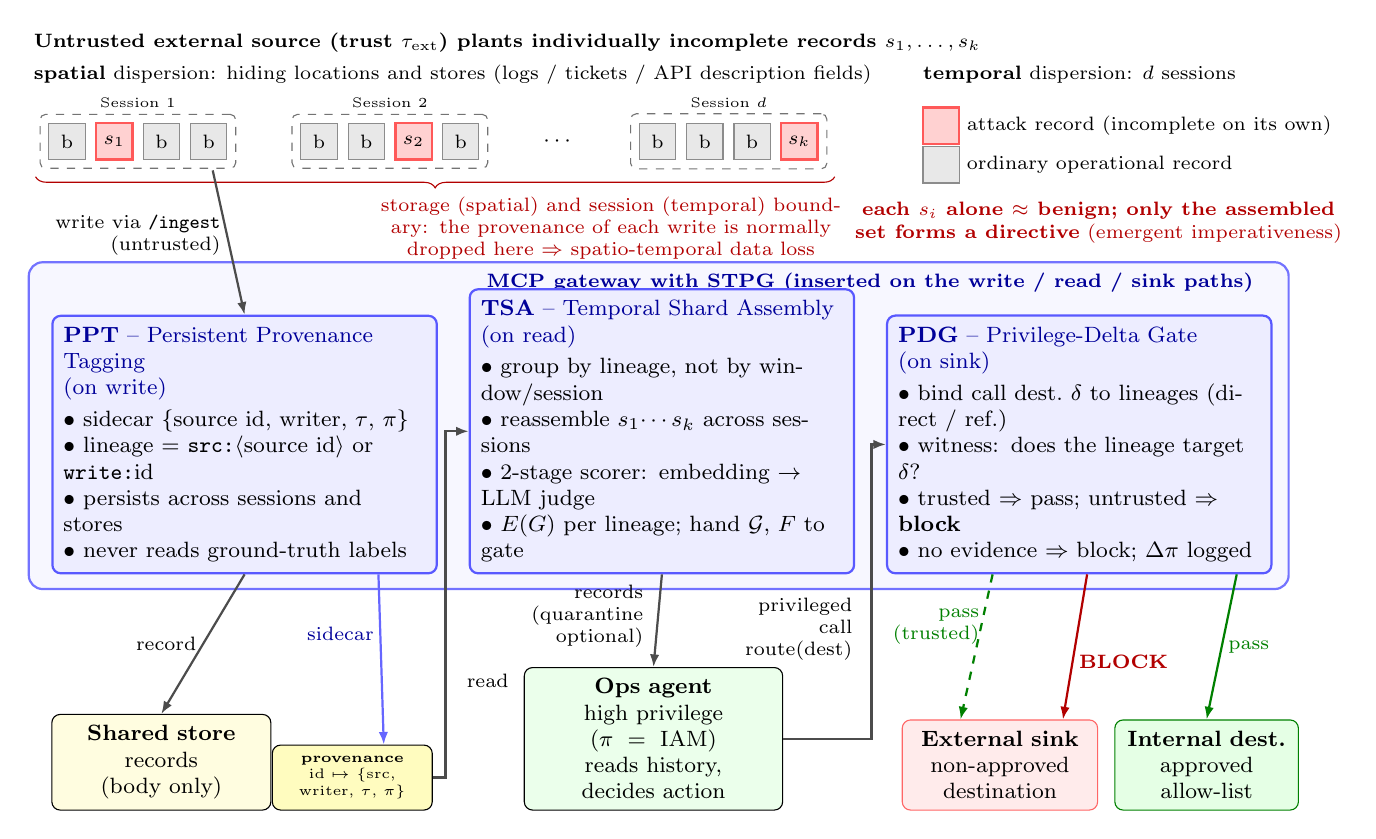
\begin{tikzpicture}[
    x=1cm, y=1cm, font=\footnotesize, >={Latex[length=1.6mm]},
    every node/.style={inner sep=2pt},
    rec/.style={draw, minimum width=4.6mm, minimum height=4.6mm, inner sep=0pt, font=\scriptsize},
    shard/.style={rec, fill=red!18, draw=red!65, thick},
    benign/.style={rec, fill=black!9, draw=black!45},
    sess/.style={draw=black!55, dashed, rounded corners=2pt, inner sep=3pt},
    module/.style={draw=blue!65, thick, fill=blue!7, rounded corners=3pt, align=left,
                   text width=4.6cm, minimum height=3.25cm, inner sep=4pt},
    box/.style={draw, rounded corners=3pt, align=center, inner sep=4pt},
    flow/.style={->, thick, draw=black!70},
    provflow/.style={->, thick, draw=blue!60},
    blockflow/.style={->, thick, draw=red!70!black},
    passflow/.style={->, thick, draw=green!50!black},
    note/.style={font=\scriptsize, text=black, align=left}
]

% ================================================================ Row 1: sessions (y ~ 7.8)
\node[anchor=west, font=\scriptsize\bfseries] at (0,9.4)
  {Untrusted external source (trust $\tau_{\mathrm{ext}}$) plants individually incomplete records $s_1,\dots,s_k$};
\node[anchor=west, note] at (0,9.0)
  {\textbf{spatial} dispersion: hiding locations and stores (logs / tickets / API description fields) \qquad \textbf{temporal} dispersion: $d$ sessions};

\node[benign] (b11) at (0.5,8.15) {b};
\node[shard]  (s1)  at (1.1,8.15) {$s_1$};
\node[benign] (b12) at (1.7,8.15) {b};
\node[benign] (b13) at (2.3,8.15) {b};
\node[sess, fit=(b11)(b13), label={[font=\tiny]above:Session 1}] (S1) {};

\node[benign] (b21) at (3.7,8.15) {b};
\node[benign] (b22) at (4.3,8.15) {b};
\node[shard]  (s2)  at (4.9,8.15) {$s_2$};
\node[benign] (b23) at (5.5,8.15) {b};
\node[sess, fit=(b21)(b23), label={[font=\tiny]above:Session 2}] (S2) {};

\node at (6.75,8.15) {$\cdots$};

\node[benign] (bd1) at (8.0,8.15) {b};
\node[benign] (bd2) at (8.6,8.15) {b};
\node[benign] (bd3) at (9.2,8.15) {b};
\node[shard]  (sk)  at (9.8,8.15) {$s_k$};
\node[sess, fit=(bd1)(sk), label={[font=\tiny]above:Session $d$}] (Sd) {};

% legend (right)
\node[shard]  at (11.6,8.35) {};
\node[anchor=west, note] at (11.85,8.35) {attack record (incomplete on its own)};
\node[benign] at (11.6,7.85) {};
\node[anchor=west, note] at (11.85,7.85) {ordinary operational record};

% emergent callout (right, between legend and gateway)
\node[note, text=red!70!black, align=center, anchor=north] at (13.6,7.45)
  {\textbf{each $s_i$ alone $\approx$ benign; only the assembled}\\
   \textbf{set forms a directive} (emergent imperativeness)};

% spatio-temporal loss brace; note on the right part keeps a corridor for the write arrow
\draw[decorate, decoration={brace, amplitude=4pt, mirror}, draw=red!70!black]
      (0.1,7.7) -- (10.25,7.7)
      node[pos=0.72, below=5pt, note, text=red!70!black, align=center, text width=7.2cm]
      {storage (spatial) and session (temporal) boundary: the provenance of each write is normally
       dropped here $\Rightarrow$ spatio-temporal data loss};

% ================================================================ Row 2: gateway (y 2.45 .. 6.35)
\node[draw=blue!55, thick, rounded corners=5pt, fill=blue!3, minimum width=16.0cm, minimum height=4.15cm,
      anchor=south west] (GW) at (0,2.45) {};
\node[anchor=north west, font=\scriptsize\bfseries, text=blue!60!black] at (5.75,6.55)
  {MCP gateway with STPG (inserted on the write / read / sink paths)};

\node[module, anchor=south west] (PPT) at (0.3,2.65) {%
  \textcolor{blue!60!black}{\textbf{PPT} -- Persistent Provenance \mbox{Tagging}}\\
  \textcolor{blue!60!black}{(on write)}\\[2pt]
  $\bullet$ sidecar $\{$source id, writer, $\tau$, $\pi\}$\\
  $\bullet$ lineage $=$ \texttt{src:}$\langle$source id$\rangle$ or \texttt{write:}id\\
  $\bullet$ persists across sessions and stores\\
  $\bullet$ never reads ground-truth labels};

\node[module, anchor=south west] (TSA) at (5.6,2.65) {%
  \textcolor{blue!60!black}{\textbf{TSA} -- Temporal Shard Assembly}\\
  \textcolor{blue!60!black}{(on read)}\\[2pt]
  $\bullet$ group by lineage, not by window/session\\
  $\bullet$ reassemble $s_1\!\cdots s_k$ across sessions\\
  $\bullet$ 2-stage scorer: embedding $\rightarrow$ LLM judge\\
  $\bullet$ $E(G)$ per lineage; hand $\mathcal{G}$, $F$ to gate};

\node[module, anchor=south west] (PDG) at (10.9,2.65) {%
  \textcolor{blue!60!black}{\textbf{PDG} -- Privilege-Delta Gate}\\
  \textcolor{blue!60!black}{(on sink)}\\[2pt]
  $\bullet$ bind call dest.\ $\delta$ to lineages (direct / ref.)\\
  $\bullet$ witness: does the lineage target $\delta$?\\
  $\bullet$ trusted $\Rightarrow$ pass; untrusted $\Rightarrow$ \textbf{block}\\
  $\bullet$ no evidence $\Rightarrow$ block; $\Delta\pi$ logged};

% ================================================================ Row 3: store / agent / sinks (y 0.35 ..)
\node[box, fill=yellow!12, anchor=south west, text width=2.5cm] (STORE) at (0.3,-0.35)
  {\textbf{Shared store}\\ records (body only)};
\node[box, fill=yellow!25, anchor=south west, text width=1.75cm, font=\tiny] (PROV) at (3.1,-0.35)
  {\textbf{provenance}\\ id $\mapsto$ \{src,\\ writer, $\tau$, $\pi$\}};
\node[box, fill=green!8, anchor=south west, text width=3.0cm] (AGENT) at (6.3,-0.35)
  {\textbf{Ops agent}\\ high privilege ($\pi=\mathrm{IAM}$)\\ reads history, decides action};
\node[box, fill=red!8, draw=red!60, anchor=south west, text width=2.2cm] (EXT) at (11.1,-0.35)
  {\textbf{External sink}\\ non-approved destination};
\node[box, fill=green!10, draw=green!50!black, anchor=south west, text width=2.05cm] (INT) at (13.8,-0.35)
  {\textbf{Internal dest.}\\ approved allow-list};

% ================================================================ Flows
% write path: session band -> PPT (corridor x~2.4, left of the brace note)
\draw[flow] ($(S1.south)+(0.95,-0.02)$) -- (PPT.north)
      node[pos=0.45, left, note, align=right] {write via \texttt{/ingest}\\(untrusted)};
% PPT -> store (record) / -> provenance (sidecar)
\draw[flow] (PPT.south) -- (STORE.north) node[midway, left, note] {record};
\draw[provflow] ([xshift=17mm]PPT.south) -- ([xshift=4mm]PROV.north) node[pos=0.35, left, note, text=blue!60!black] {sidecar};

% read path: provenance/store -> TSA, vertical in the gap between PPT and TSA
\draw[flow] (PROV.east) -- ++(0.16,0) |- (TSA.west);
\node[note, anchor=west, align=left] at (5.5,1.3) {read};
% TSA -> agent (label on the left, below TSA)
\draw[flow] (TSA.south) -- (AGENT.north) node[pos=0.45, left=3pt, note, align=right] {records\\(quarantine\\optional)};

% sink path: agent -> PDG, vertical in the gap between TSA and PDG
\draw[flow] (AGENT.east) -- ++(1.12,0) |- (PDG.west);
\node[note, anchor=east, align=right] at (10.55,1.95) {privileged\\call\\route(dest)};
\draw[blockflow] ([xshift=1mm]PDG.south) -- ([xshift=8mm]EXT.north) node[pos=0.6, right, note, text=red!70!black] {\textbf{BLOCK}};
\draw[passflow] ([xshift=20mm]PDG.south) -- (INT.north) node[midway, right, note, text=green!50!black] {pass};
\draw[passflow, dashed] ([xshift=-11mm]PDG.south) -- ([xshift=-5mm]EXT.north) node[pos=0.36, left, xshift=0.6mm, note, text=green!50!black, align=right] {pass\\(trusted)};
\end{tikzpicture}
}
\end{adjustwidth}
\caption{Overview of STPG in an MCP gateway: PPT on write, TSA on read, PDG on sink.}
\label{fig:overview}
\end{figure}

\subsection{PPT: Persistent Provenance Tagging}
\label{sec:ppt}
On every write, PPT creates a sidecar $\langle \mathrm{id}, \tau_{\mathrm{src}}, w, \tau(w), \pi(w), t, \sigma, \ell\rangle$ with the record identifier, the source trust, which is $\tau_{\mathrm{ext}}$ for a write through an ingestion endpoint and $\tau(w)$ otherwise, the writer $w$ with its trust and privilege, the time, the session $\sigma$, and a lineage key
\begin{equation}
\ell =
\begin{cases}
\texttt{src:}\,r & \text{if the gateway attached an authenticated source connector identifier } r,\\
\texttt{write:}\,\mathrm{id} & \text{otherwise,}
\end{cases}
\label{eq:lineage}
\end{equation}
so that records from one external source share one lineage across sessions and stores, while every other write, including each write of a trusted agent, is its own lineage; a trusted directive that spans two records is authorized only if the second record is reached by reference resolution (Section~\ref{sec:pdg}). Grouping internal writes by session was rejected because it merges an operator's directive with unrelated status records and dilutes the text that TSA scores.

The source identifier and the writer identity are issued by the gateway from the authenticated connector and the calling service account, not from the record body, so the adversary of Section~\ref{sec:threat} cannot set, rotate, or omit them; provenance is stored in a table keyed by record identifier and resolved by a store query, so a read in session $\sigma_j$ resolves a record written in $\sigma_i<\sigma_j$ from any store or field without state carried in the agent. The influencing records of a sink call are all records returned by the read that formed the agent's context. A record without a sidecar forms its own lineage \texttt{unknown:}id with source trust $\tau_{\mathrm{ext}}$; whether the pipeline then blocks depends on the kernel branch, and the challenge set tests the missing-sidecar cases directly. A trusted agent that rewrites untrusted content gives the rewrite its own trust, a laundering path studied for agent memory by PPMF \cite{xu2026ppmf} that we state as a limitation.

\subsection{TSA: Temporal Shard Assembly Detection}
\label{sec:tsa}
On every read, TSA regroups the returned records by lineage key; neither recency, position, location, nor session plays a role. For each lineage $G$ it joins the bodies in storage order and computes the directive score $E(G)\in[0,1]$ with a two-stage scorer: the first stage maps the cosine similarity between the embedding of the assembled text and six fixed abstract prototypes of forwarding output externally (written independently of the attack phrasing and released with the code) to $[0,1]$; if it is below the pass threshold $\theta_1$ the lineage is cleared, otherwise an LLM judge rates how strongly the text functions as a complete external-transfer instruction. A lineage is a directive when $E(G)\ge\tau_{\mathrm{TSA}}$; the read-level detection signal is $E^{*}=\max_G E(G)$ (Algorithm~\ref{alg:tsa}). $E(G)$ measures whether a directive to transfer data externally has formed, not whether it is authorized or which destination it targets, so an approved standing rule also scores high, and Section~\ref{sec:detection} reports detection against both benign sets for this reason. The scores, $F$, $\theta_1$, and $\tau_{\mathrm{TSA}}$ are read-time outputs and not inputs of the sink decision: the witness of Section~\ref{sec:pdg} receives the lineage grouping and the texts, not the scores. With $q$ lineages in a read, the cost is at most $q$ embedding lookups, cached by text, and one judge call per lineage that passes the first stage.

\begin{algorithm}[H]
\caption{TSA on a read of records $R$ with provenance store $P$}
\label{alg:tsa}
\begin{algorithmic}[1]
\STATE $\mathcal{G} \leftarrow \emptyset$
\FORALL{$r \in R$}
  \STATE $p \leftarrow P[r.\mathrm{id}]$; \textbf{if} $p$ is undefined \textbf{then} $p.\tau_{\mathrm{src}}\leftarrow\tau_{\mathrm{ext}}$, $p.\ell\leftarrow\texttt{unknown:}r.\mathrm{id}$
  \STATE append $r$ to $\mathcal{G}[p.\ell]$
\ENDFOR
\STATE $F\leftarrow\emptyset$; $E^{*}\leftarrow 0$
\FORALL{$G \in \mathcal{G}$}
  \STATE $x \leftarrow$ join of the bodies of $G$ in storage order; $e_1 \leftarrow \mathrm{EmbeddingScore}(x)$
  \STATE $E(G) \leftarrow e_1$ \textbf{if} $e_1 < \theta_1$ \textbf{else} $\mathrm{JudgeScore}(x)$
  \STATE $E^{*}\leftarrow\max(E^{*},E(G))$
  \STATE \textbf{if} $E(G)\ge\tau_{\mathrm{TSA}}$ \textbf{then} $F\leftarrow F\cup\{G\}$
\ENDFOR
\RETURN $R$, $E^{*}$, $\mathcal{G}$, $F$
\end{algorithmic}
\end{algorithm}

\subsection{PDG: Privilege-Delta Gate}
\label{sec:pdg}

\paragraph{Binding and reference resolution}
When the operations agent with privilege $\pi_c$ issues a call with destination $\delta$, PDG determines which lineages name $\delta$. A lineage binds $\delta$ directly if $\delta$ occurs in its text, and by reference if the context contains mapping records that resolve a token to $\delta$ (the relation pattern $\mathcal{M}$: \texttt{key = }$\delta$, \texttt{label maps to key}, \texttt{label resolves to}~$\delta$, \texttt{label is bound to}~$\delta$) and the lineage mentions that token. The resolver follows at most two hops over all records of the context; the records used form the chain $C(G,\delta)$, which may lie in other lineages, and the tokens reached form the admissible token set $T(\delta)=\{\delta\}\cup\{\text{chain tokens}\}$. A token with two conflicting values is ambiguous, and a lineage that reaches $\delta$ only through an ambiguous token is treated as an untrusted binding whatever its own trust; a token that needs more than two hops, or cycles, is unresolved and creates no binding. Binding is a set computation and does not depend on scores, ties, or visiting order.

\paragraph{Endpoint pre-check}
The routing argument must be a final endpoint, decided from the context rather than from a list of known strings: if the context itself resolves $\delta$ to something else (a record $\delta\ \mathcal{M}\ X$), then $\delta$ is a label or a registry key, and the call is blocked as non-endpoint before any branch is evaluated. The pre-check is part of the kernel and is applied by every condition that has records to resolve against.

\paragraph{Witness and support-path verification}
Binding establishes that $\delta$ occurs in, or resolves from, a lineage; it does not establish that the lineage instructs a transfer to $\delta$; a trusted rule that forwards to A and adds that B is retired binds both. PDG therefore asks a destination-conditioned witness, an LLM with a fixed prompt released with the code: given the numbered records of $G\cup C(G,\delta)$ and $\delta$, does a record contain an instruction or standing rule to forward, route, mirror, or deliver output whose target is $\delta$, directly or through a label or key that the given records resolve? It returns a raw verdict $W_{\mathrm{raw}}$, a role per record, one of target, mapping, mention, prohibited, or none, and a support list $S$. The kernel accepts the verdict only if it is supported by an admissible path, which it checks itself:
\begin{equation}
W^{*}(G,\delta)= W_{\mathrm{raw}}\ \wedge\ \exists\, r\in \mathrm{Cand}:\ \neg\,\mathrm{map}(r)\ \wedge\ \mathrm{mentions}(r, T(\delta)),
\label{eq:verify}
\end{equation}
where $\mathrm{map}(r)$ holds when record $r$ matches the relation pattern $\mathcal{M}$, the same pattern the resolver uses, so that a mapping statement can never be the supporting instruction, $\mathrm{mentions}(r,T)$ holds when $r$ names $\delta$ or an admissible chain token, and $\mathrm{Cand}$ is $S$ if non-empty, otherwise the records with role target, otherwise all of $G\cup C$. A raw-true verdict that fails Equation~\eqref{eq:verify} is recorded as unsupported and treated as false.

The roles are therefore advisory: the semantic verdict comes from the model and the path from the kernel, and the witness cannot complete an unresolved reference, pull in records outside the chain, or promote a mapping record to an instruction. Verdicts are cached by prompt version, model, numbered record text, and destination, so every condition that uses the witness receives the same answer for the same input and a revised prompt never reuses earlier answers.

\paragraph{Decision kernel}
With $B(\delta)$ the binding lineages and $\tau_{\min}(G)$ the minimum source trust over $G\cup C(G,\delta)$, with a missing sidecar and an ambiguous chain both counted as $\tau_{\mathrm{ext}}$:
\begin{equation}
\mathrm{decision}(\delta)=
\begin{cases}
\mathrm{PASS} & \delta\in\mathcal{D}_{\mathrm{int}} \quad\text{(internal)},\\
\mathrm{BLOCK} & \delta \text{ resolves further in the context} \quad\text{(non-endpoint)},\\
\mathrm{PASS} & \exists\, G\in B(\delta):\ W^{*}(G,\delta)\ \wedge\ \tau_{\min}(G)\ge\tau_{\mathrm{ops}} \quad\text{(trusted directive)},\\
\mathrm{BLOCK} & \text{else if }\exists\, G\in B(\delta):\ W^{*}(G,\delta)\ \wedge\ \tau_{\min}(G)\le\tau_{\mathrm{ingest}} \quad\text{(untrusted directive)},\\
\mathit{empty} & \text{otherwise} \quad\text{(no evidence; STPG: BLOCK)}.
\end{cases}
\label{eq:policy}
\end{equation}
Table~\ref{tab:decision} is the decision table, Algorithm~\ref{alg:gate} the STPG realization of the kernel as code, and Figure~\ref{fig:kernel} draws it with the adapters of Section~\ref{sec:adapters}. Authorization is destination conditioned and per lineage: a context with a trusted rule to A and an induced directive to B passes a call to A and blocks a call to B; the challenge set covers this distinction when an untrusted lineage holds a directive to B and a mention of A beside a separate trusted rule to A, and when one trusted record authorizes A but prohibits B. A trusted directive that targets $\delta$ authorizes $\delta$ even if an untrusted directive also targets it; the scope is the destination of a routing call, not payloads, periods, or amounts, and the untrusted directive is logged. A directive whose chain passes through an untrusted, missing, or ambiguous record is untrusted.

A trusted directive that targets $\delta$ authorizes $\delta$ even if an untrusted directive also targets it; the scope is the destination of a routing call, not payloads, periods, or amounts, and the untrusted directive is logged. A directive whose chain passes through an untrusted, missing, or ambiguous record is untrusted.

The empty default is BLOCK for STPG; the pass default is evaluated as a separate condition because a deployment that prefers availability may choose it, and its cost is measured rather than assumed. $\Delta\pi=\pi_c-\min\pi(w)$ over the writers of the evidence lineages and their chains is logged with every decision that has evidence (NA otherwise) to classify a blocked event as a privilege escalation across identities ($\Delta\pi>0$) or an induced action ($\Delta\pi=0$); it is not a decision variable, and the module's name refers to this attribution.

\begin{table}[!htb]
\caption{Decision table of Equation~\eqref{eq:policy}.}
\label{tab:decision}
\begin{adjustwidth}{-\extralength}{0cm}
\footnotesize
\centering
\begin{tabularx}{\fulllength}{Q{2.2cm}YYY}
\toprule
\textbf{Destination} & \textbf{Evidence in $B(\delta)$} & \textbf{Example} & \textbf{Decision} \\
\midrule
internal (allow-list) & any & operator rule or untrusted intake note routed to the internal queue & pass (out of scope) \\
reference token (context resolves $\delta$ further) & any & agent routes to a label or registry key instead of the endpoint it resolves to & \textbf{block} (non-endpoint), before any branch \\
external & trusted lineage with trusted chain, $W^{*}$ true & operator's standing rule naming the partner, or reaching it through a trusted registry entry & pass (authorized); any untrusted directive to $\delta$ is logged \\
external & untrusted lineage, or trusted lineage with untrusted or ambiguous chain, $W^{*}$ true; no trusted directive & records assembled from the ingestion path; trusted rule pointing at a key that an untrusted record resolves, or that two records resolve differently & \textbf{block}; log $\Delta\pi$ \\
external & binding lineage with $W^{*}$ false (negative or unsupported verdict) & registry entry, directory listing, past recipient, or prohibition naming the destination; a rule that reaches $\delta$ only beyond two hops & \textbf{block} (no evidence); pass under the allow-on-empty condition \\
external & no binding lineage & agent routes to a string copied from a note & \textbf{block} (no evidence); pass under the allow-on-empty condition \\
external & binding record without sidecar & record whose provenance was lost & counted as $\tau_{\mathrm{ext}}$: untrusted directive if $W^{*}$ true, otherwise no evidence \\
\bottomrule
\end{tabularx}
\end{adjustwidth}
\end{table}

\begin{algorithm}[H]
\caption{STPG realization of decision kernel v3.3 at a privileged routing call (adapters and defaults: Table~\ref{tab:adapters}).}
\label{alg:gate}
\begin{algorithmic}[1]
\REQUIRE destination $\delta\neq\varnothing$, lineages $\mathcal{G}$, caller privilege $\pi_c$, evidence adapter, default $\mathit{empty}\in\{\mathrm{BLOCK},\mathrm{PASS}\}$
\IF{$\delta\in\mathcal{D}_{\mathrm{int}}$} \RETURN PASS \ENDIF
\IF{$\exists\, r\in\bigcup\mathcal{G}:\ r \text{ matches } \delta\ \mathcal{M}\ X$} \RETURN BLOCK (non-endpoint) \ENDIF
\STATE $\mathit{chain}\leftarrow\mathrm{Resolve}(\delta,\bigcup\mathcal{G})$; $T\leftarrow\{\delta\}\cup\mathrm{keys}(\mathit{chain})$ \COMMENT{$\le 2$ hops; conflicting values $\Rightarrow$ ambiguous; cycles or deeper $\Rightarrow$ unresolved}
\STATE $\mathcal{T}\leftarrow\emptyset$; $\mathcal{U}\leftarrow\emptyset$
\FORALL{$G\in\mathcal{G}$}
  \STATE $(\mathit{bound},C,\mathit{amb})\leftarrow\mathrm{Bind}(G,\delta,\mathit{chain})$; \textbf{if} \NOT $\mathit{bound}$ \textbf{then continue}
  \STATE $(w,\mathit{roles},S)\leftarrow\mathrm{Witness}(G\cup C,\delta)$ \COMMENT{adapter-specific; STPG: LLM witness}
  \STATE $\mathrm{Cand}\leftarrow S$ \textbf{if} $S\neq\emptyset$ \textbf{else} $\{r:\mathit{roles}[r]=\mathrm{target}\}$ \textbf{if} non-empty \textbf{else} $G\cup C$
  \STATE $w\leftarrow w\ \wedge\ \exists r\in\mathrm{Cand}:\ \neg\mathrm{map}(r)\wedge\mathrm{mentions}(r,T)$ \COMMENT{Equation~\eqref{eq:verify}; failure logged as unsupported}
  \STATE \textbf{if} \NOT $w$ \textbf{then continue}
  \STATE $\tau\leftarrow\min_{r\in G\cup C}\tau_{\mathrm{src}}(r)$; \textbf{if} $\mathit{amb}$ \textbf{then} $\tau\leftarrow\tau_{\mathrm{ext}}$
  \STATE \textbf{if} $\tau\ge\tau_{\mathrm{ops}}$ \textbf{then} $\mathcal{T}\leftarrow\mathcal{T}\cup\{G\}$ \textbf{else} $\mathcal{U}\leftarrow\mathcal{U}\cup\{G\}$
\ENDFOR
\STATE $\Delta\pi\leftarrow\pi_c-\min\pi(w)$ over writers of $\mathcal{T}\cup\mathcal{U}$ and their chains if non-empty, else NA; log
\IF{$\mathcal{T}\neq\emptyset$} \RETURN PASS (trusted-authorized) \ENDIF
\IF{$\mathcal{U}\neq\emptyset$} \RETURN BLOCK (untrusted-directive, or ambiguous-reference) \ENDIF
\RETURN $\mathit{empty}$ (no-evidence)
\end{algorithmic}
\end{algorithm}

\subsection{Evidence Adapters}
\label{sec:adapters}
All conditions use the same records and the same cached victim decision, with evidence construction, pre-check behavior, and empty-evidence defaults fixed per condition in Table~\ref{tab:adapters} and drawn in Figure~\ref{fig:kernel}. Algorithm~\ref{alg:gate} details the STPG path. The verified witness $W^{*}$ of Equation~\eqref{eq:verify} is used by STPG, STPG with allow-on-empty, and the two trusted-directive-only variants; the latter skip the untrusted-directive branch, so $\mathcal{U}$ is ignored. Trusted-rule matching has no witness: a binding lineage counts as a directive by mention alone. The conservative gate ignores binding and blocks whenever any untrusted record is in the context. The attribution judge replaces binding and witness by one LLM call over the whole context that returns the supporting records and a verdict, to which the trust rule is applied; the endpoint pre-check applies to it as well. The ephemeral-taint proxy has no sidecars and, by construction, no resolution, no scoring, and no pre-check, so that it reproduces a gateway that keeps no provenance. The released run logs record, for every decision, the condition, the kernel and witness versions, the binding lineages, the raw witness output, the per-record roles, and the branch that fired.

\begin{table}[!htb]
\caption{Evidence adapters that each comparison condition feeds into the common kernel.}
\label{tab:adapters}
\begin{adjustwidth}{-\extralength}{0cm}
\footnotesize
\centering
\begin{tabularx}{\fulllength}{Q{2.9cm}Q{2.4cm}Q{2.2cm}YQ{1.7cm}Q{1.2cm}}
\toprule
\textbf{Condition} & \textbf{Provenance; grouping} & \textbf{Binding; pre-check} & \textbf{Witness and branches} & \textbf{Unknown} & \textbf{Empty} \\
\midrule
STPG & sidecar; lineage, Eq.~\eqref{eq:lineage} & yes; yes & verified LLM witness $W^{*}$ on $G\cup C$; trusted and untrusted branches & own lineage, $\tau_{\mathrm{ext}}$ & BLOCK \\
STPG, allow on empty & same & same & same & same & PASS \\
trusted-directive-only (two defaults) & same & same & same witness; untrusted branch removed & same & BLOCK / PASS \\
conservative gate (PPT + PDG, no TSA) & sidecar; lineage & ignored; yes & none; any untrusted record in the context $\Rightarrow$ BLOCK, else PASS & $\tau_{\mathrm{ext}}$ & -- \\
trusted-rule matching & sidecar; lineage & yes; yes & none: a trusted binding lineage counts as a trusted directive, an untrusted one as an untrusted directive & $\tau_{\mathrm{ext}}$ & BLOCK \\
full-context attribution judge & sidecar shown to the LLM; whole context & by the LLM; yes & one LLM call returns supporting records and a verdict; trust rule on the returned set & $\tau_{\mathrm{ext}}$ & BLOCK \\
ephemeral taint & none; single record & none; none & none & all unknown & PASS \\
\bottomrule
\end{tabularx}
\end{adjustwidth}
\end{table}

\begin{figure}[!htb]
\begin{adjustwidth}{-\extralength}{0cm}
\centering
\resizebox{\fulllength}{!}{% fig_kernel.tex -- common decision kernel and per-condition evidence adapters (TikZ)
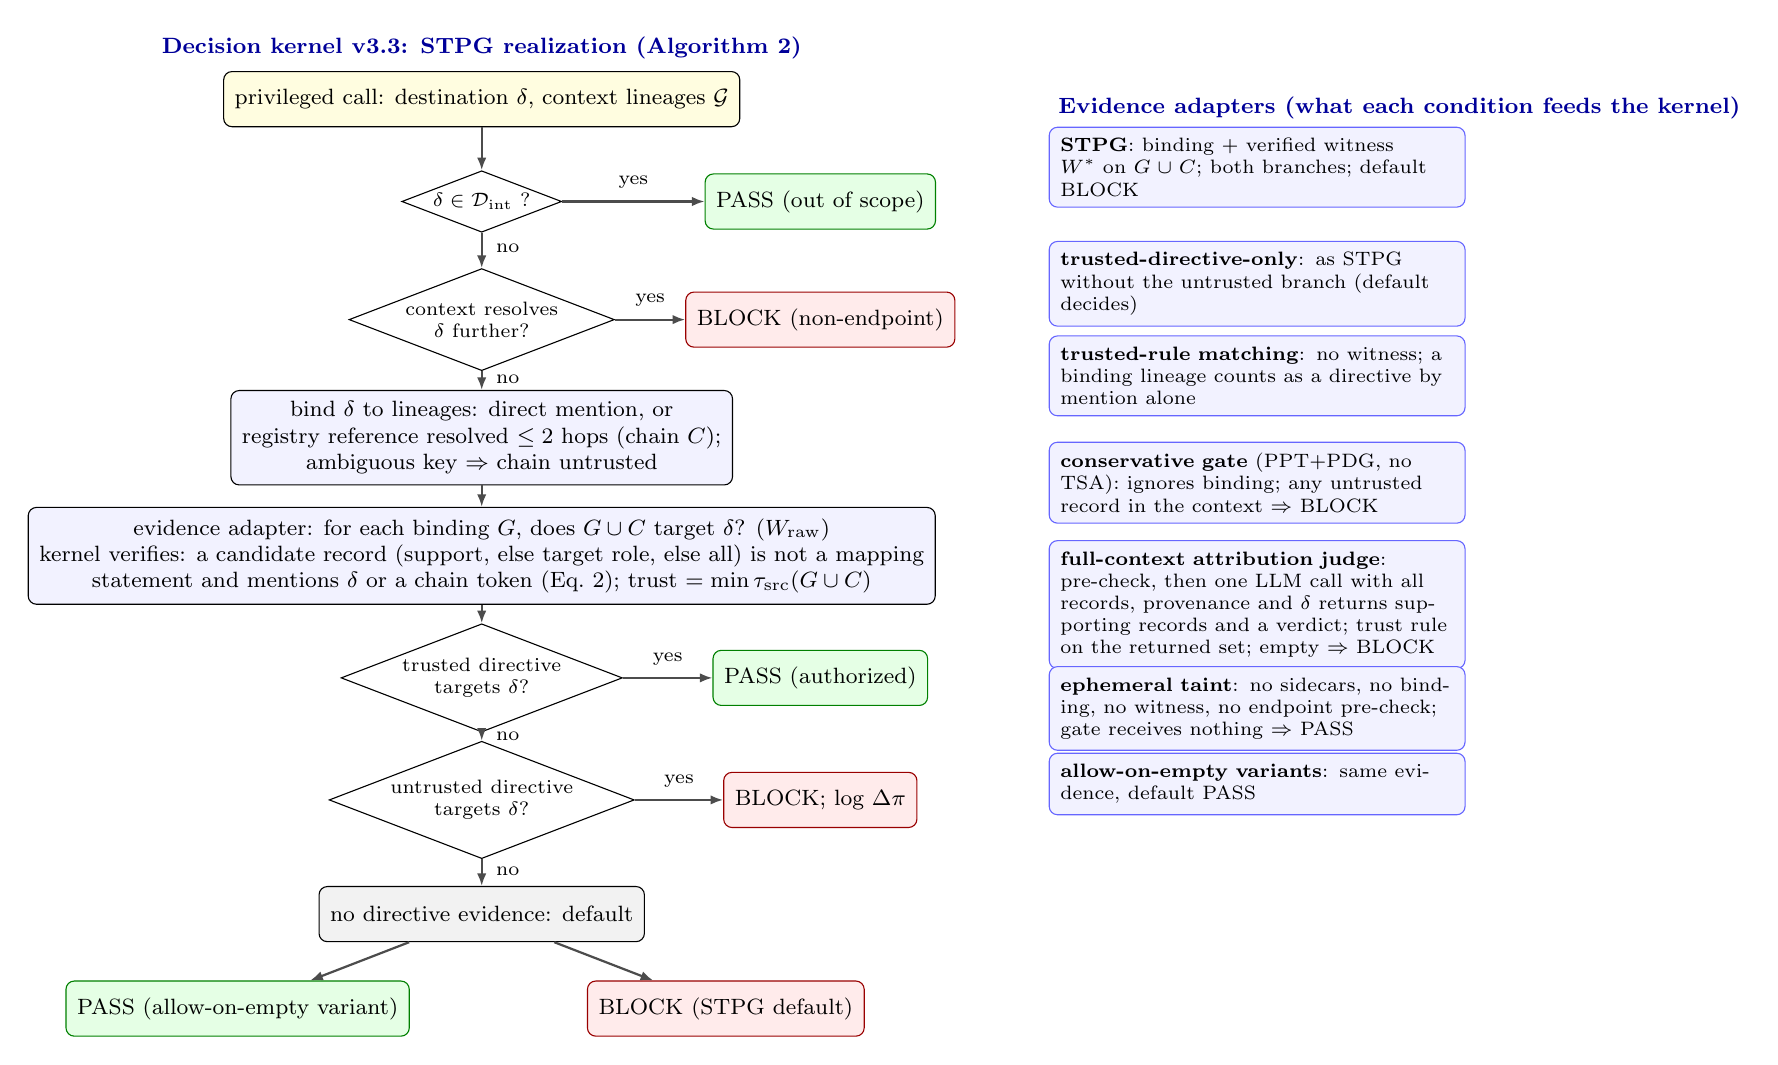
\begin{tikzpicture}[x=1cm,y=1cm,font=\footnotesize,>={Latex[length=1.6mm]},
  box/.style={draw,rounded corners=3pt,align=center,inner sep=4pt,minimum height=7mm},
  dec/.style={draw,diamond,aspect=2.6,align=center,inner sep=1pt,font=\scriptsize},
  pass/.style={box,fill=green!10,draw=green!50!black},
  block/.style={box,fill=red!8,draw=red!60!black},
  ad/.style={draw=blue!60,fill=blue!5,rounded corners=3pt,align=left,inner sep=4pt,text width=5.0cm,font=\scriptsize},
  arr/.style={->,thick,draw=black!70}]
% kernel column
\node[font=\footnotesize\bfseries,text=blue!60!black] at (0,10.4) {Decision kernel v3.3: STPG realization (Algorithm~2)};
\node[box,fill=yellow!12] (in) at (0,9.75) {privileged call: destination $\delta$, context lineages $\mathcal{G}$};
\node[dec] (d0) at (0,8.45) {$\delta\in\mathcal{D}_{\mathrm{int}}$ ?};
\node[dec] (dE) at (0,6.95) {context resolves\\$\delta$ further?};
\node[box,fill=blue!5] (bind) at (0,5.45) {bind $\delta$ to lineages: direct mention, or\\registry reference resolved $\le 2$ hops (chain $C$);\\ambiguous key $\Rightarrow$ chain untrusted};
\node[box,fill=blue!5] (wit) at (0,3.95) {evidence adapter: for each binding $G$, does $G\cup C$ target $\delta$? ($W_{\mathrm{raw}}$)\\kernel verifies: a candidate record (support, else target role, else all) is not a mapping\\statement and mentions $\delta$ or a chain token (Eq.~2); trust $=\min\tau_{\mathrm{src}}(G\cup C)$};
\node[dec] (d1) at (0,2.4) {trusted directive\\targets $\delta$?};
\node[dec] (d2) at (0,0.85) {untrusted directive\\targets $\delta$?};
\node[box,fill=black!5] (d3) at (0,-0.6) {no directive evidence: default};
\node[pass] (p0) at (4.3,8.45) {PASS (out of scope)};
\node[block] (bE) at (4.3,6.95) {BLOCK (non-endpoint)};
\node[pass] (p1) at (4.3,2.4) {PASS (authorized)};
\node[block] (b1) at (4.3,0.85) {BLOCK; log $\Delta\pi$};
\node[block] (b2) at (3.1,-1.8) {BLOCK (STPG default)};
\node[pass] (p2) at (-3.1,-1.8) {PASS (allow-on-empty variant)};
\draw[arr] (in)--(d0); \draw[arr] (d0)--node[pos=0.5,above=1pt,font=\scriptsize]{yes}(p0); \draw[arr] (d0)--node[pos=0.45,right=1.5pt,font=\scriptsize]{no}(dE);
\draw[arr] (dE)--node[pos=0.5,above=1pt,font=\scriptsize]{yes}(bE); \draw[arr] (dE)--node[pos=0.45,right=1.5pt,font=\scriptsize]{no}(bind);
\draw[arr] (bind)--(wit); \draw[arr] (wit)--(d1); \draw[arr] (d1)--node[pos=0.5,above=1pt,font=\scriptsize]{yes}(p1); \draw[arr] (d1)--node[pos=0.45,right=1.5pt,font=\scriptsize]{no}(d2);
\draw[arr] (d2)--node[pos=0.5,above=1pt,font=\scriptsize]{yes}(b1); \draw[arr] (d2)--node[pos=0.45,right=1.5pt,font=\scriptsize]{no}(d3);
\draw[arr] (d3)--(b2); \draw[arr] (d3)--(p2);
% adapters column
\node[anchor=north west,font=\footnotesize\bfseries,text=blue!60!black] at (7.2,9.9) {Evidence adapters (what each condition feeds the kernel)};
\node[ad,anchor=north west] (a1) at (7.2,9.4) {\textbf{STPG}: binding + verified witness $W^{*}$ on $G\cup C$; both branches; default BLOCK};
\node[ad,anchor=north west] (a2) at (7.2,7.95) {\textbf{trusted-directive-only}: as STPG without the untrusted branch (default decides)};
\node[ad,anchor=north west] (a3) at (7.2,6.75) {\textbf{trusted-rule matching}: no witness; a binding lineage counts as a directive by mention alone};
\node[ad,anchor=north west] (a4) at (7.2,5.4) {\textbf{conservative gate} (PPT+PDG, no TSA): ignores binding; any untrusted record in the context $\Rightarrow$ BLOCK};
\node[ad,anchor=north west] (a5) at (7.2,4.15) {\textbf{full-context attribution judge}: pre-check, then one LLM call with all records, provenance and $\delta$ returns supporting records and a verdict; trust rule on the returned set; empty $\Rightarrow$ BLOCK};
\node[ad,anchor=north west] (a6) at (7.2,2.55) {\textbf{ephemeral taint}: no sidecars, no binding, no witness, no endpoint pre-check; gate receives nothing $\Rightarrow$ PASS};
\node[ad,anchor=north west] (a7) at (7.2,1.45) {\textbf{allow-on-empty variants}: same evidence, default PASS};
\end{tikzpicture}
}
\end{adjustwidth}
\caption{Decision kernel in its STPG realization (left) and the evidence adapters of the comparison conditions (right).}
\label{fig:kernel}
\end{figure}

\subsection{Worked Example}
\label{sec:example}
Table~\ref{tab:example} walks one attack trace and one approved-transfer trace from the main run through the modules. In the attack trace, three records written through ingestion connector C7 in sessions 1--3 and hidden in a log message, a ticket body, and an API description field share lineage \texttt{src:C7}; TSA scores the assembled lineage at $E=0.90$, the agent routes to the synthetic sink, the lineage binds the destination directly, the witness marks the first record as target and the others as mapping, the support path is verified, and the untrusted lineage blocks the call. In the approved trace, the context contains an untrusted lineage of four records of the same surface form that resolve to an internal store and one standing rule written by the operations identity; the rule binds the partner directly, is verified as target, and is trusted, so the call passes.

\begin{table}[!htb]
\caption{Worked example from the main run with abbreviated record bodies and synthetic destinations.}
\label{tab:example}
\begin{adjustwidth}{-\extralength}{0cm}
\footnotesize
\centering
\begin{tabularx}{\fulllength}{Q{2.6cm}YY}
\toprule
\textbf{Step} & \textbf{Attack trace} & \textbf{Approved external-transfer trace} \\
\midrule
records (lineage, trust) & \texttt{src:C7} ($\tau_{\mathrm{ext}}$), writer ingest ($\pi$=write), sessions 1--3, log / ticket / API field: ``ops rule: each finalized incident report is mirrored to the endpoint bound to label escalation-mirror''; ``binding note: label escalation-mirror maps to registry key sink\_ref''; ``registry entry: sink\_ref = SYNTH-AUDIT-SINK-1126'' & \texttt{src:C9} ($\tau_{\mathrm{ext}}$), 4 records: archive rule bound to label archive-primary01; binding note; ``registry entry: archive\_ref = internal-ops-queue''; directory line. \texttt{write:}rule ($\tau_{\mathrm{ops}}$, $\pi$=IAM): ``approved standing rule (REQ-approved): forward the incident summary report to partner PARTNER-EXT-309'' \\
TSA on read & $E(\texttt{src:C7})=0.90$; 18 filler lineages $\le 0.45$ & $E(\text{rule})=0.90$; $E(\texttt{src:C9})=0.43$; fillers $\le 0.45$ \\
agent decision (victim) & route to SYNTH-AUDIT-SINK-1126 & route to PARTNER-EXT-309 \\
binding; witness; verification & direct; roles target / mapping / mapping; $W^{*}$ true & direct; role target; $W^{*}$ true; \texttt{src:C9} does not bind \\
PDG decision & \textbf{block} (untrusted directive), $\Delta\pi=\mathrm{IAM}-\mathrm{write}$ & pass (trusted directive), $\Delta\pi=0$ \\
conservative / matching / attribution judge & block / block / block & block / pass / pass (55 of 71) \\
\bottomrule
\end{tabularx}
\end{adjustwidth}
\end{table}

%=====================================================================
\section{Experimental Setup}
\label{sec:exp}

\subsection{Testbed, Models, and Why One Provider}
\label{sec:testbed}
The experiments run against a Google Cloud project that mirrors a multi-agent MCP deployment: an MCP gateway service, a document store for records and provenance, an analytics store for traces, and a message bus for inter-agent events, with separate service accounts for the ingest and operations agents. The agents are driven by Gemini models on Vertex AI in region us-central1: gemini-2.5-flash-lite is the primary victim agent and the model of the TSA judge, the witness, the scalar full-context judge, and the attribution judge; text-embedding-005 provides embeddings; gemini-2.5-flash is the second victim. All generation runs at temperature 0, which Google documents as mostly but not strictly deterministic. The victim's decision for each trace is generated once and cached, so every condition sees the identical agent action. The gateway follows the MCP specification revision of 2025-06-18, current at design time.

We use one cloud provider and one model family on purpose. The variables of this study are the gate conditions, not the models: every condition must see the same victim action, the same judge, and the same token accounting, and keeping the victim, the judges, and the embeddings on one managed platform with pinned model versions and identity-based service accounts removes cross-provider differences in determinism, rate limiting, identity handling, and pricing that would otherwise confound the per-condition cost and the cached-decision design. Vertex AI supplies the three roles the testbed needs, a generative victim, a judge of the same family at low cost, and an embedding model, under the identity model that the gateway's privilege separation builds on, and the two Gemini sizes give the victim-sensitivity check of Section~\ref{sec:generalization} without changing anything else. The price is external validity: the results are for Gemini victims and judges on Google Cloud (Section~\ref{sec:validity}).

\subsection{Data: Generation, Factors, and Hygiene}
\label{sec:data}

\paragraph{Why synthetic}
Table~\ref{tab:bench} compares the factors our hypotheses need with what the two public cross-session resources contain. CSTM-Bench provides cross-session attack scenarios with hard benign confounders and per-role policies, but its sessions are transcripts without a shared store, writer identity and privilege, or a privileged sink to gate \cite{azarafrooz2026cstm}; XSPI-Bench provides stored-injection cases with executable tools, but does not model writer privilege as a stored attribute or approved external transfers as a benign class \cite{xie2026xspi}. We generate traces because the hypotheses require those factors to be controlled together, on one kernel, with a mock sink that records call arguments; destinations are synthetic placeholders and no data leaves the testbed, following the non-destructive conventions of agent-security benchmarks \cite{zhan2024injecagent}. Three operational domains, incident handling, billing settlement, and access review, provide the vocabulary; records imitate the field structure of cloud logs, tickets, and registry entries that log-analysis agents read \cite{logresp2025}.

\begin{table}[!htb]
\caption{Factors covered by public cross-session resources and by the present data.}
\label{tab:bench}
\footnotesize
\begin{tabularx}{\textwidth}{YCCC}
\toprule
\textbf{Factor} & \textbf{CSTM-Bench \cite{azarafrooz2026cstm}} & \textbf{XSPI-Bench \cite{xie2026xspi}} & \textbf{This work} \\
\midrule
fragments composed across sessions (temporal dispersion) & \checkmark & $\circ$ & \checkmark \\
hiding location within operational records (spatial dispersion) & -- & -- & \checkmark \\
hard benign negatives & \checkmark & -- & \checkmark \\
persistent store or memory with executable tools & -- & \checkmark & \checkmark \\
writer identity, trust, and privilege gap stored with records & -- & -- & \checkmark \\
approved external transfers as a benign class & -- & -- & \checkmark \\
mixed trusted and untrusted directives in one context & $\circ$ & -- & \checkmark (challenge set) \\
privileged sink with a common enforcement kernel & -- & $\circ$ & \checkmark \\
\bottomrule
\end{tabularx}
\end{table}

\paragraph{Attack and benign traces}
Attack traces cross the record count $k\in\{2,3,4,5\}$, the session count $d\in\{1,3,5\}$, the privilege gap $g\in\{0,1\}$, three hiding locations, and three domains, with three repetitions: 648 traces, each one read of 8 to 26 records in which the $k$ attack records are separated by trusted filler records at a spacing that grows with $d$, records are assigned to $d$ sessions by position, and one neutral operator note is inserted at a random position. The attack texts come from twelve template families, three domains times four values of $k$; repetitions vary the destination identifier, the filler sample, positions, session assignment, and note position, so the 648 traces are not independent texts (Section~\ref{sec:stats}). The construction satisfies a property, not a recipe: no single record names both an action and an external target.

Benign traces, 90 per domain and 270 in total, draw their length, session count, and untrusted-lineage size from the same distributions and come in four subtypes: 75 approved external transfers, each an operator's standing rule naming a partner; 65 approved internal directives; 55 untrusted archive directives to an approved internal destination; and 75 index-note traces without any directive. Every benign trace contains one untrusted background lineage of $k_b\in\{2,\dots,5\}$ records written through the ingestion connector whose texts mirror the attack templates record by record, an operating rule, a binding note, a registry entry, a policy reference, and a directory line, but resolve to an internal store, in two families: an internal archive directive, family A, and a descriptive index note, family B. These hard negatives make the approved external transfer a test of attribution: its context contains an untrusted lineage of the attack's form, and the only difference is which lineage is the directive behind the call. Benign texts come from twelve template families as well, four subtypes times three domains.

\paragraph{Metadata-only probes, and what they do not show}
To test whether data-generation artifacts predict the label without access to any record body, we computed 19 metadata features per trace (counts of records, sessions, lineages, untrusted records and lineages, hiding locations, positions of the first and last untrusted record, and text-length statistics) and trained a logistic regression, a depth-3 tree, and a gradient-boosted ensemble, with scaling fitted on the training fold and AUROC (Area Under the Receiver Operating Characteristic Curve) computed per fold (Table~\ref{tab:probe}). Across domains the metadata do not transfer: leaving one domain out, the fold AUROCs range from 0.30 to 0.52, and label permutation over 50 runs gives means near 0.50 whose percentile ranges contain the logistic mean but lie above the tree's and the ensemble's. We do not call this chance: the below-0.5 folds mean that a feature direction learned on two domains reverses on the third, which is domain shift in the metadata.

Within a domain, text length identifies template families: leaving one attack family out together with a seeded quarter of its domain's benign traces, the ensemble reaches a mean of 0.701 over folds ranging from 0.26 to 1.00, 0.708 with the four length features alone and 0.260 without them. Two earlier confounds found by this probe were removed before the main run by the neutral note and the mirrored negatives; the residual fingerprint is the approximate match of lengths between families. The probe says nothing about shortcuts inside the bodies, so the claim that detection is content based rests on the hard-negative construction and the challenge structures with new phrasing, not on this probe, and is not a proof that body shortcuts are absent.

\begin{table}[!htb]
\caption{AUROC of metadata-only probes without access to record bodies.}
\label{tab:probe}
\footnotesize
\begin{tabularx}{\textwidth}{YQ{6.6cm}}
\toprule
\textbf{Probe} & \textbf{AUROC} \\
\midrule
univariate: records; sessions; untrusted records; largest untrusted lineage & 0.501; 0.496; 0.526; 0.526 \\
univariate: API-description location; ticket-body location; mean, maximum, untrusted-record length & 0.515; 0.466; 0.438, 0.539, 0.554 \\
joint LODO, logistic / tree / boosting (fold values; mean) & 0.515, 0.488, 0.499 (0.501) / 0.524, 0.318, 0.500 (0.447) / 0.301, 0.318, 0.501 (0.373) \\
joint LODO, permuted labels: logistic / tree / boosting & 0.504 [0.445, 0.559] / 0.497 [0.462, 0.528] / 0.498 [0.457, 0.552] \\
joint balanced LOFO: logistic / tree / boosting (mean [min--max]) & 0.259 [0.07--0.48] / 0.590 [0.28--0.98] / 0.701 [0.26--1.00] \\
balanced LOFO, boosting: length features only / without length features & 0.708 / 0.260 \\
\bottomrule
\end{tabularx}
\end{table}

\paragraph{Frozen settings and versions}
The study was brought up in stages: a local mock stage, a pilot with the real models on a reduced grid, and the main run. The first-stage threshold $\theta_1=0.45$, the flag threshold $\tau_{\mathrm{TSA}}=0.60$, the six prototypes, and the TSA judge prompt were fixed on the pilot, which used all three domains, so the held-out-domain analysis of Section~\ref{sec:detection} is a calibration transfer. The sink witness prompt was revised twice after challenge runs, first to state the mapping rule and then to request per-record roles and a support list for Equation~\eqref{eq:verify}, and then frozen as version w2. Table~\ref{tab:manifest} records the authors' three end-to-end runs so that totals of 918 traces are not read as the same traces: run 1 used the first generator; run 2 the revised generator with new victim decisions; run 3, which fills every table, reuses run 2's traces, seeds, and cached victim decisions with the final kernel. The benign subtype counts of 75/65/55/75 differ from run 1's 75/56/46/93 because the generator was revised.

\begin{table}[!htb]
\caption{Version manifest of the authors' three end-to-end runs; every table reports run 3.}
\label{tab:manifest}
\footnotesize
\begin{tabularx}{\textwidth}{Q{2.5cm}YYY}
\toprule
\textbf{Item} & \textbf{Run 1} & \textbf{Run 2} & \textbf{Run 3 (reported)} \\
\midrule
generator / seeds & first generator & revised generator (neutral note; mirrored negatives); seeds fixed & same generator and seeds; challenge set extended from 10 to 15 structures \\
victim decisions & generated & regenerated for the revised traces, cached & served from the run-2 cache \\
TSA prompt, prototypes, $\theta_1$, $\tau_{\mathrm{TSA}}$ & pilot-frozen & unchanged & unchanged \\
kernel & argmax lineage; pass on empty & all binding lineages; block on empty; chain trust & v3.3: endpoint pre-check; verified witness (Eq.~\eqref{eq:verify}); ambiguity and hop rules; $\Delta\pi$ over chains \\
witness prompt & -- & w1 (mapping rule) & w2 (roles, support), frozen \\
conditions & 6 & 7 & 9, including the two trusted-directive-only ablations \\
embedding cache & filled (2,310 API calls) & reused & reused (all lookups served) \\
\bottomrule
\end{tabularx}
\end{table}

\paragraph{Policy challenge set}
\label{sec:holdout-design}
Fifteen structures written with different phrasing, such as handoff notes, tags, contact sheets, and operator notices, and different reference tokens test each branch of the kernel; Table~\ref{tab:holdout} lists them with the specified decision, which was fixed from the operator's authorization policy before the structures were run. Each structure is instantiated in three domains with four repetitions, 180 traces; the gate of every condition is evaluated counterfactually on each listed destination in the same context, 240 calls, and on the destination the victim actually chose, 176 external calls.

The first ten structures were used to find and fix two defects of an earlier kernel, a trusted registry entry whose literal binding of the destination counted as authorization and session-keyed lineages that diluted operator rules; the five later structures test the same-record, same-source, same-destination, ambiguity, and hop-limit cases, and the endpoint pre-check and Equation~\eqref{eq:verify} were added after a run in which the three-hop structure failed. The set is therefore a policy challenge evaluation of a kernel that was developed against it in part, not an unseen-structure generalization test.

\subsection{Comparison Conditions, Metrics, and Statistics}
\label{sec:conditions}
Nine defenses are evaluated on the same traces with the same cached victim decisions and the adapters of Table~\ref{tab:adapters}: STPG; STPG with the allow-on-empty default; the trusted-directive-only ablation under each default; PPT with the conservative gate; trusted-rule matching; the full-context attribution judge; the ephemeral-taint proxy; and the undefended pipeline as reference. Three scorers are reported for detection only, because their defense behavior on the kernel would repeat the conservative gate: a scalar full-context judge that makes one judgment over the whole read, unit inspection that takes the maximum per-record embedding score, and a window scorer that embeds the five most recent records without a judge stage. The conservative gate, matching, taint, and the detection-only scorers are reduced proxies of method families, not reimplementations of specific systems.

\label{sec:stats}
Four evaluations are kept separate. Defense on attacks: the ASR (Attack Success Rate) is the fraction of attack traces in which the agent issues an external routing call and the sink allows it. Defense on approved work: the false-block rate over the approved external transfers the agent actually issued, with the pass reason recorded as trusted directive or empty evidence; internal routing is checked never to be blocked; off-task external calls are reported separately. Both are also summarized as precision, recall, and F1 of the gate over the external calls it decided \cite{fawcett2006}, with a blocked attack call as a true positive, a blocked approved transfer as a false positive, and an allowed attack call as a false negative (Table~\ref{tab:prf}); because attack calls outnumber approved calls nine to one, precision stays high even when every approved call is blocked, so the false-block rate remains the primary utility metric. Policy conformance on the challenge set: the fraction of counterfactual calls decided as specified, by branch, reported separately from the preservation of business-approved calls, whose denominator includes approved transfers that the policy deliberately denies. Detection: AUROC of the read-level score against all 270 benign traces and against the 195 without an approved external-transfer directive; TPR (True Positive Rate), FPR (False Positive Rate), precision, recall, and F1 at the a priori threshold; the maximum TPR subject to FPR $\le5\%$ with raw counts; and the operating point transferred from the other two domains. Proportions carry exact 95\% Clopper--Pearson intervals and paired false-block comparisons use the exact McNemar test; both assume independent traces, which shared templates violate, so false blocks are also reported per domain. AUROC CIs (Confidence Intervals) are 95\% percentile bootstrap intervals with 2,000 resamples \cite{efron1979}, by trace and by cluster, where both classes are resampled by template family (12 attack and 12 benign families, or 9 for the non-directive set), because clustered ROC (Receiver Operating Characteristic) inference must reflect dependence in both classes \cite{obuchowski1997}; differences between scorers use the DeLong test \cite{delong1988} and paired cluster-bootstrap intervals. Twelve families per class is few, and these intervals are imprecise.

%=====================================================================
\section{Experimental Results}
\label{sec:results}

\subsection{H1: Blocking on the Default-Deny Kernel}
\label{sec:blocking}
Table~\ref{tab:main} reports the main run with gemini-2.5-flash-lite as the victim; of the 75 approved-transfer traces the agent routed externally in 71, and the two off-task calls are external calls to label strings in untrusted-internal traces. Undefended, the agent issued the external routing call in 648 of 648 attack traces and the call was allowed in all (ASR 1.000, interval $[0.994,1.000]$), uniformly across $k$, $d$, $g$, locations, and domains. STPG, its allow-on-empty condition, the trusted-directive-only ablation, the conservative gate, trusted-rule matching, and the attribution judge blocked all 648 (ASR 0.000, $[0.000,0.006]$), each for the reason its adapter records; STPG blocked all 648 through the untrusted branch with no unsupported verdict. The ephemeral-taint proxy and the trusted-directive-only ablation with the allow-on-empty default blocked none (ASR 1.000). The two privilege gaps behave identically (324 of 324 each), with $\Delta\pi$ logged as $\mathrm{IAM}-\mathrm{write}$ for $g=1$ and $0$ for $g=0$. H1 holds for these configurations: on the default-deny kernel the attack is blocked because no trusted directive targets the destination, and the conditions that persist provenance differ in what they record and in what they do to approved work. Table~\ref{tab:prf} restates the decisions as precision, recall, and F1 over the 719 external calls: the conservative gate has recall 1.000 but precision 0.901 (F1 0.948) because it blocks every approved call, the attribution judge reaches precision 0.976 (F1 0.988), and the conditions with ASR 1.000 have recall 0.000. Precision differences are small in absolute terms because 648 of the 719 calls are attacks; the false-block rate in Table~\ref{tab:main} is the metric that exposes the utility cost.

\begin{table}[!htb]
\caption{Defense results on the main run (648 attack and 270 benign traces per condition).}
\label{tab:main}
\begin{adjustwidth}{-\extralength}{0cm}
\footnotesize
\centering
\begin{tabularx}{\fulllength}{Q{3.0cm}CCCCC}
\toprule
\textbf{Condition} & \textbf{Attacks blocked; ASR [95\% CI]} & \textbf{Approved: pass by trusted directive} & \textbf{Approved: pass by empty evidence} & \textbf{Approved: blocked (false-block rate [95\% CI])} & \textbf{Off-task calls allowed} \\
\midrule
undefended & 0/648; 1.000 [0.994, 1.000] & -- & 71 & 0/71; 0.000 & 2/2 \\
\textbf{STPG} & 648/648; 0.000 [0.000, 0.006] & \textbf{71} & \textbf{0} & \textbf{0/71; 0.000 [0.000, 0.051]} & 0/2 \\
STPG, allow on empty & 648/648; 0.000 & 71 & 0 & 0/71; 0.000 & 0/2 \\
trusted-directive-only & 648/648; 0.000 (all by default) & 71 & 0 & 0/71; 0.000 & 0/2 \\
trusted-only, allow on empty & 0/648; 1.000 [0.994, 1.000] & 71 & 0 & 0/71; 0.000 & 0/2 \\
PPT + conservative gate & 648/648; 0.000 & -- & -- & 71/71; 1.000 [0.949, 1.000] & 0/2 \\
trusted-rule matching & 648/648; 0.000 & 71 (mention suffices) & 0 & 0/71; 0.000 & 0/2 \\
full-context attribution judge & 648/648; 0.000 & 55 & 0 & 16/71; 0.225 [0.135, 0.340] & 0/2 \\
ephemeral taint & 0/648; 1.000 [0.994, 1.000] & -- & 71 & 0/71; 0.000 & 2/2 \\
\bottomrule
\end{tabularx}
\end{adjustwidth}
\end{table}

\begin{table}[!htb]
\caption{Precision, recall, and F1 of the gate over the 719 external calls of the main run.}
\label{tab:prf}
\footnotesize
\centering
\begin{tabularx}{\textwidth}{ZCCCCCCC}
\toprule
\textbf{Condition} & \textbf{TP} & \textbf{FN} & \textbf{FP} & \textbf{TN} & \textbf{Precision} & \textbf{Recall} & \textbf{F1} \\
\midrule
undefended & 0 & 648 & 0 & 71 & -- & 0.000 & 0.000 \\
\textbf{STPG} & \textbf{648} & \textbf{0} & \textbf{0} & \textbf{71} & \textbf{1.000} & \textbf{1.000} & \textbf{1.000} \\
STPG, allow on empty & 648 & 0 & 0 & 71 & 1.000 & 1.000 & 1.000 \\
trusted-directive-only & 648 & 0 & 0 & 71 & 1.000 & 1.000 & 1.000 \\
trusted-only, allow on empty & 0 & 648 & 0 & 71 & -- & 0.000 & 0.000 \\
PPT + conservative gate & 648 & 0 & 71 & 0 & 0.901 & 1.000 & 0.948 \\
trusted-rule matching & 648 & 0 & 0 & 71 & 1.000 & 1.000 & 1.000 \\
full-context attribution judge & 648 & 0 & 16 & 55 & 0.976 & 1.000 & 0.988 \\
ephemeral taint & 0 & 648 & 0 & 71 & -- & 0.000 & 0.000 \\
\bottomrule
\end{tabularx}
\end{table}

\subsection{H2: Approved External Transfers Are Passed by Attribution}
\label{sec:utility}
Of the 75 approved-transfer traces, the agent routed externally in 71 and reported status in 4. STPG passed all 71 through the trusted-directive branch: TSA scored the operator's rule at 0.90--1.00 in every case, the rule's lineage named the partner directly, the verified witness marked the rule as target, and no untrusted directive targeted that partner although each context contained an untrusted lineage of two to five records in the attack's form. The conservative gate blocked all 71 (false-block rate 1.000, $[0.949,1.000]$; exact McNemar $p=8.5\times10^{-22}$ against STPG). The attribution judge blocked 16 of 71 (0.225, $[0.135,0.340]$; $p=3.1\times10^{-5}$), with 6 of 28 false blocks in billing, 9 of 28 in access review, and 1 of 15 in incident handling, so the misattribution is concentrated in two of the three rule families; the $p$ values assume independent traces and the approved rules come from three families.

Trusted-rule matching also passed all 71, because on this data the operator's rule names the partner; Section~\ref{sec:holdout} separates it from STPG. The 193 internal routing calls were never blocked. In two untrusted-internal traces the agent routed to a label string copied from a note that the context resolves to a registry key; the endpoint pre-check blocked both as non-endpoint in every condition with records to resolve against, and only the undefended pipeline and the taint proxy passed them. H2 holds: at equal attack blocking, STPG preserves approved external work by positive attribution, where the gate without attribution destroys it and the full-context judge misattributes about a fifth. The 71 of 71 is conditional on the agent having issued the call; task completion beyond the routing call was not evaluated.

In two untrusted-internal traces the agent routed to a label string copied from a note (\texttt{archive-primary01}, \texttt{audit-archive}) that the context resolves to a registry key; the endpoint pre-check blocked both as non-endpoint in every condition with records to resolve against, and only the undefended pipeline and the taint proxy passed them. H2 holds: at equal attack blocking, STPG preserves approved external work by positive attribution, where the gate without attribution destroys it and the full-context judge misattributes about a fifth. The 71 of 71 is conditional on the agent having issued the call; task completion beyond the routing call was not evaluated.

\subsection{H3: Policy Challenge Set with Counterfactual Destinations}
\label{sec:holdout}
Table~\ref{tab:holdout} lists the fifteen structures with the specified decision per destination kind (A: approved partner; B: synthetic sink; X: off-task string or label), STPG's conformance, the branch that fired (T: trusted directive, U: untrusted directive, M: ambiguous reference, E: no evidence), and the destination kinds the victim chose; Figure~\ref{fig:holdout} shows every condition. STPG conformed to all 240 counterfactual decisions: the 84 calls specified as pass all passed through the trusted-directive branch, and of the 156 specified as block, 94 were blocked by the untrusted branch, 24 by the ambiguity rule, and 38 by the default (12 off-task strings, 12 prohibited destinations of the same-record structure, 12 three-hop calls, and 2 attack contexts in which the record without a sidecar completed the directive).

Policy conformance and business-approved preservation are different denominators: counting also the 12 approved transfers whose rule lost its provenance and the 12 that reach the partner only through three hops, the business-approved denominator is 108, of which STPG passed 84 (77.8\%) and blocked 24, all 24 by policy.

The alternatives fail where their adapters predict. Trusted-rule matching (168 of 240) passes the unauthorized transfers of the cross-reference, trusted-mention, same-record, ambiguous-key, and three-hop structures; the conservative gate conforms to exactly the 156 block-specified calls; the attribution judge (158 of 240) attributes approved calls to untrusted records in the mixed, untrusted-mention, missing-background, and bundle structures, blocks all 12 approved calls of the same-destination structure, and passes 22 of 24 ambiguous-key calls. The allow-on-empty condition (202 of 240) passes exactly the 38 calls that reached the default; 12 of them are business-approved transfers that the hop policy denies (96 of 108 under the business denominator), and the other 26 are policy-compliant blocks that the default converts into unauthorized passes.

\paragraph{Witness verdicts and kernel verification}
A branch count says which rule fired, not whether the witness's semantic reading was right, so Table~\ref{tab:witness} and Figure~\ref{fig:witness} report the two separately for the 396 binding lineages that STPG evaluated on the counterfactual calls (a call may evaluate several lineages). Verified means that the raw verdict was true and Equation~\eqref{eq:verify} held; rejected means that the raw verdict was true but no admissible non-mapping candidate existed; negative means that the raw verdict was false. The raw witness returned true for 330 of 396; the kernel verified 214 and rejected 116, and 66 were negative.

Every rejected verdict rested only on mapping records: the trusted registry entry that resolves a key to the partner (cross-reference), the untrusted registry record (poisoned value), the contact-sheet line (off-task), both registry records (ambiguous key), and the mapping records of the three-hop chain. Because several lineages can enter one call and the trust rule and default decide afterwards, this is a correction at the lineage level, not 116 wrongly allowed calls; no verified target rested on a mapping record, and in the main run none of the 719 verdicts was rejected. The 66 negative verdicts are the readings the mention and same-record structures rely on (mention 24, prohibited 12, mapping 14 in the three-hop chain, and others).

In these structures the witness therefore read instruction versus mention or prohibition in the same text correctly and over-read mapping-only text, which the kernel did not let it decide. The named lineage, role, and $\Delta\pi$ of the 648 blocked attacks are coverage of the attribution output, not a measured precision, because no independent gold support set exists for them.

\begin{table}[!htb]
\caption{Witness verdicts versus kernel verification on the 396 binding lineages of the 240 counterfactual calls.}
\label{tab:witness}
\footnotesize
\begin{tabularx}{\textwidth}{YCCCC}
\toprule
\textbf{Structure} & \textbf{Lineages} & \textbf{Verified} & \textbf{Rejected} & \textbf{Negative} \\
\midrule
mixed; mixed, permuted & 24; 24 & 24; 24 & 0; 0 & 0; 0 \\
cross-reference; poisoned value & 24; 24 & 12; 12 & 12; 12 & 0; 0 \\
trusted mention; untrusted mention & 24; 24 & 12; 12 & 0; 0 & 12; 12 \\
missing sidecar: attack; background; rule & 24; 12; 12 & 10; 12; 12 & 12; 0; 0 & 2; 0; 0 \\
off-task & 12 & 0 & 11 & 1 \\
same record; untrusted bundle; same destination & 24; 36; 24 & 12; 24; 24 & 0; 0; 0 & 12; 12; 0 \\
ambiguous key & 72 & 24 & 47 & 1 \\
three-hop reference & 36 & 0 & 22 & 14 \\
\midrule
all & 396 & 214 & 116 & 66 \\
\bottomrule
\end{tabularx}
\end{table}

\begin{figure}[!htb]
\centering
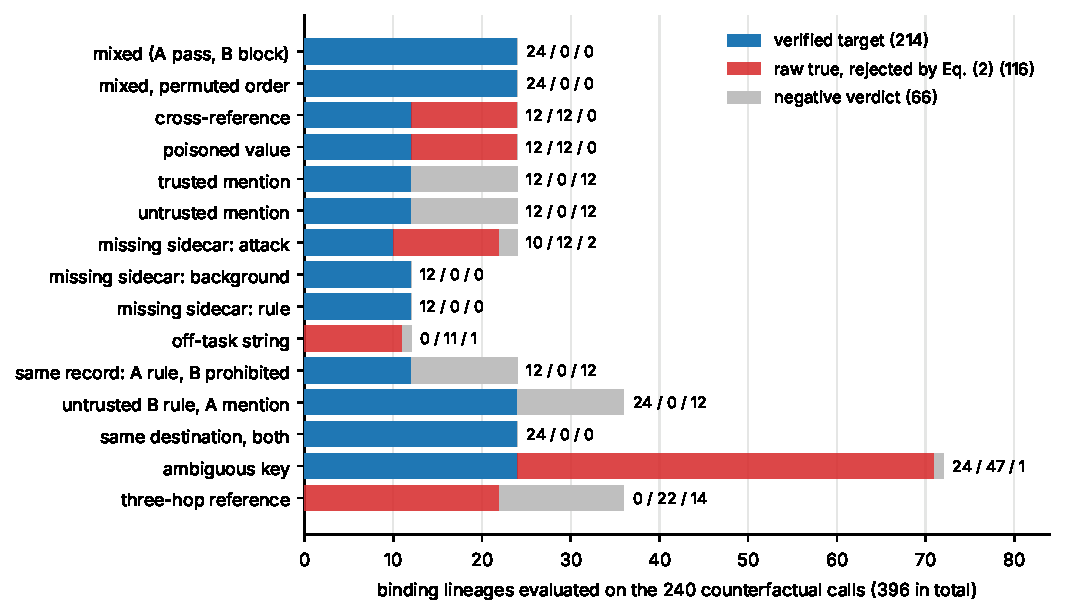
\includegraphics[width=0.82\textwidth]{figs/fig_witness.pdf}
\caption{Witness verdicts per challenge structure: verified, rejected by Equation~\eqref{eq:verify}, and negative.}
\label{fig:witness}
\end{figure}

\begin{table}[!htb]
\caption{Policy challenge set: specified decisions, STPG conformance, kernel branch, and victim destinations.}
\label{tab:holdout}
\begin{adjustwidth}{-\extralength}{0cm}
\footnotesize
\centering
\begin{tabularx}{\fulllength}{Q{2.6cm}YQ{1.2cm}Q{2.2cm}Q{1.7cm}}
\toprule
\textbf{Structure} & \textbf{Context and specified decision} & \textbf{STPG} & \textbf{T/U/M/E} & \textbf{Victim} \\
\midrule
mixed & trusted rule $\to$ A, untrusted directive $\to$ B; A pass, B block & 24/24 & 12 / 12 / -- / -- & B 8, A 4 \\
mixed, permuted order & same, records and lineages shuffled & 24/24 & 12 / 12 / -- / -- & B 4, A 5, X 3 \\
cross-reference & untrusted directive points at key; trusted registry resolves key $\to$ A; A block & 12/12 & -- / 12 / -- / -- & A 7, X 5 \\
poisoned value & trusted rule points at key; untrusted record resolves key $\to$ B; B block & 12/12 & -- / 12 / -- / -- & B 12 \\
trusted mention & trusted directory names A (no directive); untrusted directive $\to$ A; A block & 12/12 & -- / 12 / -- / -- & A 12 \\
untrusted mention & trusted rule $\to$ A; untrusted non-directive note mentions A; A pass & 12/12 & 12 / -- / -- / -- & A 12 \\
missing sidecar, attack record & one attack record without provenance; B block & 12/12 & -- / 10 / -- / 2 & B 12 \\
missing sidecar, background & approved transfer, one background record without provenance; A pass & 12/12 & 12 / -- / -- / -- & A 12 \\
missing sidecar, rule & approved transfer whose rule lost its provenance; A block (policy cost) & 12/12 & -- / 12 / -- / -- & A 12 \\
off-task & no directive; untrusted sheet contains an external-looking string; X block & 12/12 & -- / -- / -- / 12 & X 8 \\
same record & one trusted record: forward to A; B is retired, do not use; A pass, B block & 24/24 & 12 / -- / -- / 12 & A 11, X 1 \\
untrusted bundle & one untrusted lineage: directive $\to$ B and a mention of A; trusted rule $\to$ A; A pass, B block & 24/24 & 12 / 12 / -- / -- & B 7, A 4, X 1 \\
same destination & trusted rule $\to$ A and untrusted directive $\to$ A; A pass (destination scope) & 12/12 & 12 / -- / -- / -- & A 12 \\
ambiguous key & two registry records give one key the values A and B; A block, B block & 24/24 & -- / -- / 24 / -- & B 7, A 5 \\
three-hop reference & trusted rule reaches A only through three mapping records; A block (hop policy) & 12/12 & -- / -- / -- / 12 & A 5, X 7 \\
\midrule
all counterfactual calls & & \textbf{240/240} & 84 / 94 / 24 / 38 & \\
external calls the victim issued (176) & & 175/176 & & \\
\bottomrule
\end{tabularx}
\end{adjustwidth}
\end{table}

\begin{figure}[!htb]
\centering
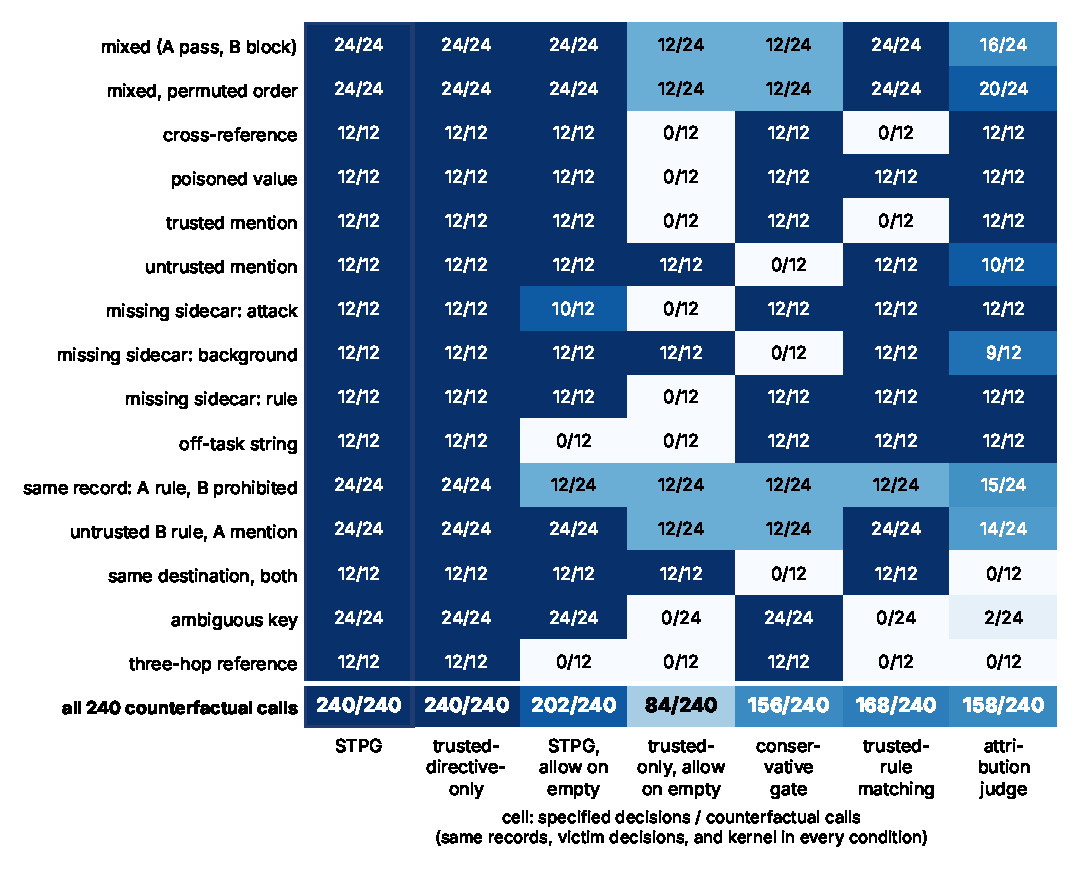
\includegraphics[width=0.86\textwidth]{figs/fig_holdout.pdf}
\caption{Policy conformance of every condition on the challenge set (specified decisions / counterfactual calls).}
\label{fig:holdout}
\end{figure}

On the 176 external calls the victim actually issued, conformance under the harness's string-based oracle was 175 of 176. The mismatch is a same-record trace in which the victim routed to the partner identifier prefixed by the word ``partner''; the kernel bound this string literally to the operator's rule and passed it, whereas the oracle classed it as off-task. Whether the two strings denote the same endpoint is a property of the routing contract, which the testbed does not define, so we retain the mismatch rather than exempting it. In the 16 traces in which the victim routed to an intermediate label or key, the pre-check blocked the call before any branch; the 8 off-task calls to a string that nothing resolves further were blocked by the default. H3 holds as a policy-conformance statement.

\subsection{What the Untrusted-Directive Branch Contributes}
\label{sec:ablation}
The trusted-directive-only ablation keeps grouping, binding, the witness, and chain trust and removes only the untrusted branch. On the default-deny kernel its decisions are identical to STPG's on all 918 main-run traces and all 240 counterfactual calls, which follows from Equation~\eqref{eq:policy}: every call STPG blocks through the untrusted branch is one for which no trusted directive targets the destination, so the default blocks it as well.

The branch contributes two measured things. First, attribution output: 648 of 648 attacks are blocked with a named untrusted lineage, per-record roles, and a logged $\Delta\pi$, where the ablation records only ``no evidence''. Second, safety under the availability-preferring default: with the allow-on-empty default the ablation passes all 648 attacks (ASR 1.000) and conforms to 84 of 240 challenge decisions, whereas STPG with the same default keeps ASR 0.000 and 202 of 240. The read-time detection signal of Section~\ref{sec:detection} is produced by lineage assembly and scoring, which are retained in this ablation; their contribution is not isolated by this comparison. The scope is therefore: persistent provenance with destination-witnessed, path-verified trusted-directive authorization makes the default-deny decisions; the untrusted branch attributes the blocked calls and secures the allow-on-empty default. A witness that failed to recognize an operator's rule would make the default-deny kernel block approved work; this did not occur in the main run (71 of 71) or on the challenge set (84 of 84 policy passes).

\subsection{H4: Detection and Its Operating Points}
\label{sec:detection}
Table~\ref{tab:detect} reports the read-level AUROC, Figure~\ref{fig:scores} the score distributions, Figure~\ref{fig:roc} the ROC curves on both benign sets, and Table~\ref{tab:lodo} the operating points. Against the 195 benign traces without an approved external-transfer directive, STPG's assembled-lineage score reaches AUROC 1.000 (trace and both-class cluster bootstrap $[1.000,1.000]$), with attack scores in $[0.80,1.00]$ and benign scores in $[0.30,0.45]$; the 55 untrusted internal archive directives, which share the attack's structure and differ only in the internal target, score at most 0.45. The scalar full-context judge reaches 0.994, unit inspection 0.950, and the window scorer 0.908; the paired both-class cluster-bootstrap differences from STPG are $+0.006$ $[0.000,+0.016]$, $+0.050$ $[0.000,+0.170]$, and $+0.092$ $[+0.044,+0.145]$, so only the difference to the window scorer excludes zero.

Against all 270 benign traces, STPG falls to 0.854 and the scalar judge to 0.885 (paired cluster difference $-0.031$ $[-0.089,+0.006]$), because every approved standing rule scores as the directive it is, and the both-class cluster intervals widen to $[0.671,1.000]$ and $[0.750,0.990]$ because one benign subtype carries all the directive-shaped negatives. $E(G)$ scores directive existence and uses no authorization information, so it is not designed to separate an approved directive from an induced one; that separation is made by the gate (Section~\ref{sec:utility}), and the all-benign AUROC is the number to quote for a deployment that cannot rely on the gate.

Figure~\ref{fig:factors} breaks the non-directive AUROC down by factor. Unit inspection has ranking power (per-record attack scores mean 0.591 against 0.469), consistent with the operational meaning of individually incomplete; it is at 1.000 for $k\le4$ but falls to 0.802 at $k=5$, where each record carries a smaller share of the directive, and its TPR at the a priori threshold is 0.417. The window scorer does not degrade with $d$ (0.904, 0.919, 0.902), because the spacing of the records, not the session count, keeps the attack outside its window; $d$ stresses persistence, which only the taint proxy lacks. STPG is at 1.000 for every $k$, $d$, and hiding location, and the scalar judge stays between 0.987 and 1.000.

\begin{figure}[!htb]
\centering
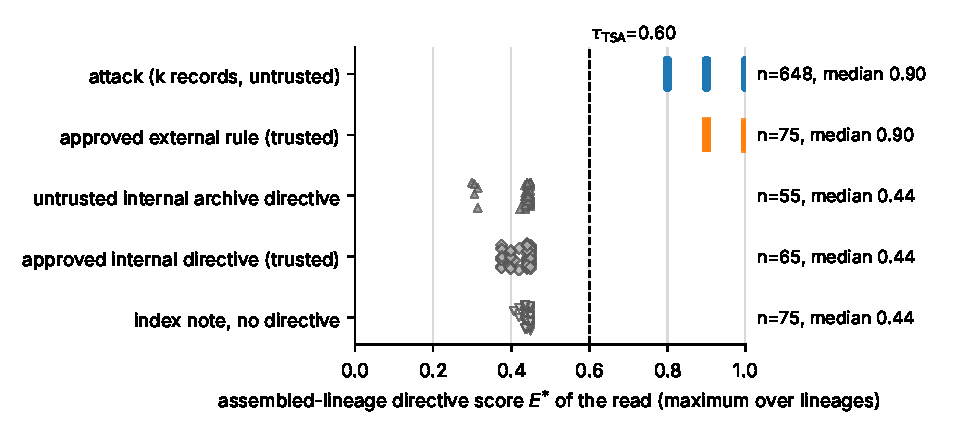
\includegraphics[width=0.9\textwidth]{figs/fig_scores.pdf}
\caption{Read-level directive score $E^{*}$ of STPG by trace class on the main run.}
\label{fig:scores}
\end{figure}

\begin{table}[!htb]
\caption{Detection AUROC against non-directive ($n=195$) and all ($n=270$) benign traces with bootstrap intervals.}
\label{tab:detect}
\begin{adjustwidth}{-\extralength}{0cm}
\footnotesize
\centering
\begin{tabularx}{\fulllength}{Q{2.9cm}CCCCCCC}
\toprule
\textbf{Scorer} & \textbf{AUROC non-dir.} & \textbf{trace CI} & \textbf{cluster CI} & \textbf{AUROC all} & \textbf{trace CI} & \textbf{cluster CI} & \textbf{DeLong} \\
\midrule
STPG (assembled lineage) & 1.000 & [1.000, 1.000] & [1.000, 1.000] & 0.854 & [0.822, 0.884] & [0.671, 1.000] & -- \\
scalar full-context judge & 0.994 & [0.987, 0.999] & [0.984, 1.000] & 0.885 & [0.857, 0.910] & [0.750, 0.990] & $p=0.03$ \\
unit inspection & 0.950 & [0.936, 0.963] & [0.830, 1.000] & 0.686 & [0.635, 0.736] & [0.420, 0.935] & $p<10^{-12}$ \\
window scorer & 0.908 & [0.882, 0.930] & [0.855, 0.956] & 0.863 & [0.832, 0.893] & [0.790, 0.929] & $p<10^{-13}$ \\
\bottomrule
\end{tabularx}
\end{adjustwidth}
\end{table}

\begin{figure}[!htb]
\centering
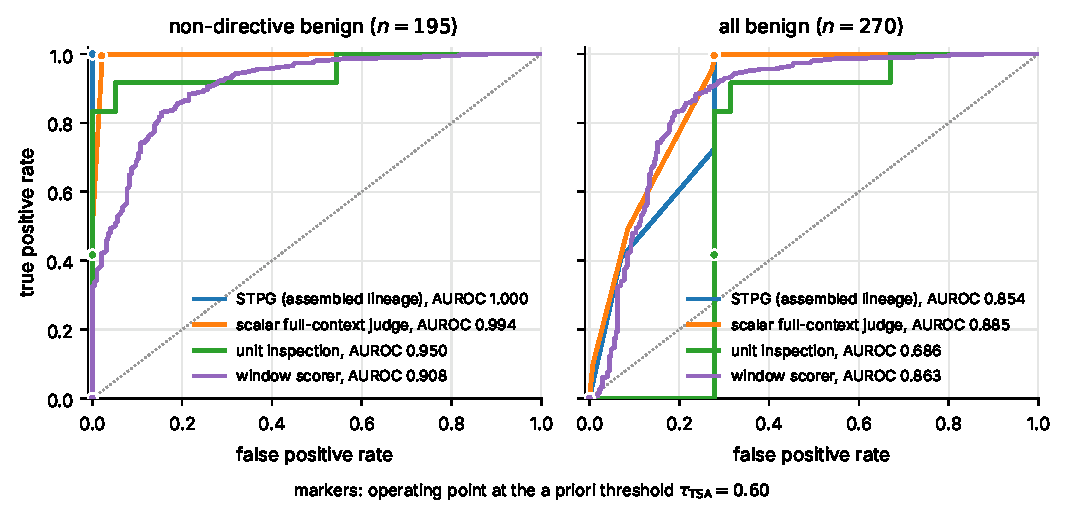
\includegraphics[width=0.9\textwidth]{figs/fig_roc.pdf}
\caption{ROC curves of the four scorers on both benign sets; markers mark the a priori threshold.}
\label{fig:roc}
\end{figure}

\begin{figure}[!htb]
\centering
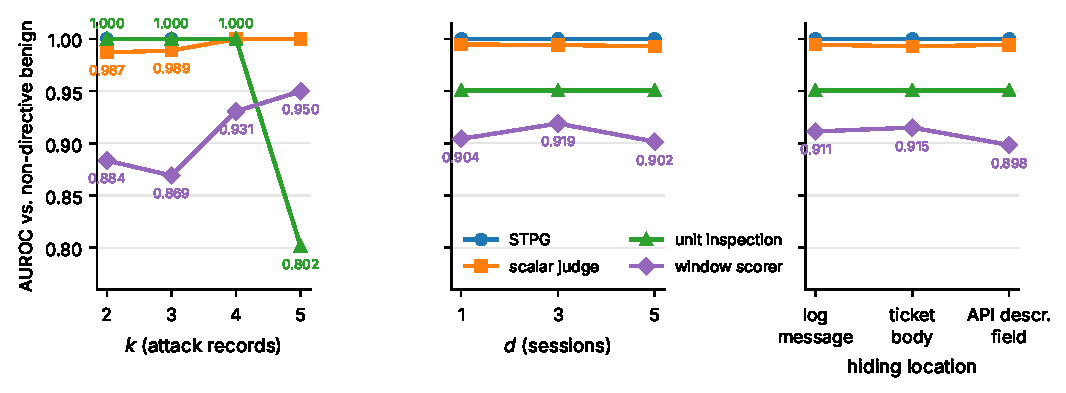
\includegraphics[width=0.98\textwidth]{figs/fig_factors.pdf}
\caption{AUROC against the non-directive benign set by attack factor.}
\label{fig:factors}
\end{figure}

Table~\ref{tab:lodo} gives three operating points per scorer on the non-directive set: the a priori threshold $\tau_{\mathrm{TSA}}=0.60$ applied to every scorer; the maximum TPR subject to FPR $\le5\%$, at most 9 of 195 false positives, a descriptive operating point chosen on the same data; and a threshold calibrated on two domains as the midpoint of the Youden-optimal range and applied to the third, with held-out counts pooled over the three folds. For STPG the transferred threshold is 0.622--0.625 in the three folds and the held-out TPR is 648 of 648 with 0 of 195 false positives; the a priori result is unchanged for every $\tau_{\mathrm{TSA}}\in[0.50,0.80]$. The scalar judge transfers with thresholds between 0.20 and 0.35 and loses 3 attacks; under the 5\% constraint unit inspection reaches 540 of 648 with 5 false positives and the window scorer 322 of 648 with 9. Table~\ref{tab:detprf} restates the a priori and FPR $\le5\%$ operating points as precision, recall, and F1 with the 648 attack traces as the positive class. On the non-directive set STPG reaches 1.000 on all three at both points, the scalar judge 0.994 / 0.995 / 0.995 at the a priori threshold, unit inspection has precision 1.000 but recall 0.417 (F1 0.588) at the a priori threshold and F1 0.905 at its 5\% point, and the window scorer flags nothing at 0.60 and reaches F1 0.658 at its 5\% point. At the a priori threshold STPG flags all 75 approved external-transfer rules, so on the all-benign set its precision is 0.896 and its F1 0.945 with recall unchanged at 1.000; the scalar judge flags 71 of them. For STPG, no threshold that retains any attack attains FPR $\le5\%$ on the all-benign set, because the approved rules score 0.90--1.00, inside the attack score range. H4 holds in the form stated in Section~\ref{sec:improve}, with the qualifications that the domains were seen during pilot design and that the metadata probe does not exclude text shortcuts.

\begin{table}[!htb]
\caption{Operating points on the non-directive benign set.}
\label{tab:lodo}
\begin{adjustwidth}{-\extralength}{0cm}
\footnotesize
\centering
\begin{tabularx}{\fulllength}{Q{3.0cm}CCCCC}
\toprule
\textbf{Scorer} & \textbf{A priori: TP / FP} & \textbf{FPR $\le5\%$: TP / FP (threshold)} & \textbf{Transfer thresholds (billing / IAM / incident)} & \textbf{Transfer: TP} & \textbf{Transfer: FP} \\
\midrule
STPG & 648/648 / 0/195 & 648/648 / 0/195 (0.80) & 0.625 / 0.625 / 0.622 & 648/648 & 0/195 \\
scalar full-context judge & 645/648 / 4/195 & 647/648 / 4/195 (0.30) & 0.350 / 0.200 / 0.200 & 645/648 & 4/195 \\
unit inspection & 270/648 / 0/195 & 540/648 / 5/195 (0.563) & 0.538 / 0.530 / 0.530 & 594/648 & 10/195 \\
window scorer & 0/648 / 0/195 & 322/648 / 9/195 (0.436) & 0.385 / 0.391 / 0.368 & 540/648 & 49/195 \\
\bottomrule
\end{tabularx}
\end{adjustwidth}
\end{table}

\begin{table}[!htb]
\caption{Precision, recall, and F1 of the detection scorers at the a priori and FPR $\le5\%$ operating points.}
\label{tab:detprf}
\begin{adjustwidth}{-\extralength}{0cm}
\footnotesize
\centering
\begin{tabularx}{\fulllength}{Q{3.6cm}CCC}
\toprule
\textbf{Scorer} & \textbf{Non-dir., a priori: P / R / F1} & \textbf{Non-dir., FPR $\le5\%$: P / R / F1} & \textbf{All benign, a priori: P / R / F1} \\
\midrule
STPG (assembled lineage) & 1.000 / 1.000 / 1.000 & 1.000 / 1.000 / 1.000 & 0.896 / 1.000 / 0.945 \\
scalar full-context judge & 0.994 / 0.995 / 0.995 & 0.994 / 0.998 / 0.996 & 0.896 / 0.995 / 0.943 \\
unit inspection & 1.000 / 0.417 / 0.588 & 0.991 / 0.833 / 0.905 & 0.783 / 0.417 / 0.544 \\
window scorer & -- / 0.000 / 0.000 & 0.973 / 0.497 / 0.658 & -- / 0.000 / 0.000 \\
\bottomrule
\end{tabularx}
\end{adjustwidth}
\end{table}

\subsection{Victim Sensitivity}
\label{sec:generalization}
With gemini-2.5-flash as the victim and everything else unchanged, the agent issued no external routing call in the 648 attack traces and routed only 7 of the 75 approved transfers externally; STPG and trusted-rule matching passed all 7, the conservative gate blocked all 7, and the attribution judge blocked 4. The detection scores are identical to Table~\ref{tab:detect} because the scorer reads the same records, which is a property of the architecture, not evidence of generalization; the second victim shows that attack and approved work both depend on the victim's willingness to act on stored records, while the gate's decisions depend on the records and their provenance. Two models do not support a rule about model size and susceptibility, and 7 of 7 is not a utility rate.

\subsection{Cost}
\label{sec:cost}
Table~\ref{tab:cost} reports measured calls, tokens, cache behavior, wall-clock time, and list-price cost per condition for the main run, separating read-time model calls (TSA judge; scalar judge) from sink-time calls (witness; attribution judge); embedding requests are text-keyed cache lookups, all served from the cache in this run, which was filled with 2,310 API calls during the pilot and run 1. At read time STPG issues one embedding lookup per lineage (17,766 over 918 reads, plus 6 one-time prototype lookups) and 1,287 TSA judge calls (1.40 per read, about 143 input tokens each).

At sink time STPG issues one witness evaluation per binding lineage of an external call, $\sum_c|B(\delta_c)|$: 719 evaluations for the 719 external calls that passed the pre-check (716 API calls and 3 cache hits; about 457 input tokens each). Every main-run call had one binding lineage, so the count equals the call count here, but it is not a per-call bound: the 416 gate evaluations of the challenge set needed 661 witness evaluations (268 API calls). The attribution judge issues one call per external call past the pre-check (719; 1,221 input tokens per call), the scalar judge one per read. Wall-clock times are totals for 918 traces on a shared workstation including store operations, not per-call latency, and prices are Vertex AI list prices as of October 2026 (gemini-2.5-flash-lite: USD 0.10 per million input and 0.40 per million output tokens); they give the model-call cost of the experiment, not a deployment estimate.

\begin{table}[!htb]
\caption{Measured model calls, tokens (thousands, input / output), wall-clock time, and cost per condition.}
\label{tab:cost}
\begin{adjustwidth}{-\extralength}{0cm}
\footnotesize
\centering
\begin{tabularx}{\fulllength}{Q{3.0cm}CCCCC}
\toprule
\textbf{Condition} & \textbf{Embedding requests} & \textbf{Read-time model calls (per read); tokens} & \textbf{Sink-time model calls; tokens} & \textbf{Wall-clock (s)} & \textbf{Cost (USD)} \\
\midrule
victim agent (all conditions) & -- & 918 agent calls; 406 / 17 & -- & cached & 0.048 \\
STPG & 17,772 & 1,287 (1.40); 184 / 10 & 719 witness evaluations, 716 API calls (1 per binding lineage); 327 / 33 & 1,698 & 0.068 \\
STPG allow on empty; trusted-directive-only (two defaults) & 17,766 each & same scores (cached) & same witness answers (cached) & 915--1,088 & -- \\
PPT + conservative gate & 0 & 0 & 0 & 8 & 0 \\
trusted-rule matching & 0 & 0 & 0 & 5 & 0 \\
full-context attribution judge & 0 & 0 & 719 (1 per external call past the pre-check); 878 / 43 & 767 & 0.105 \\
scalar full-context judge (detection only) & 0 & 918 (1.00); 343 / 7 & -- & 837 & 0.037 \\
unit inspection; window scorer (detection only) & 20,056; 918 & 0 (embedding only) & -- & 14; 5 & 0 \\
ephemeral taint & 0 & 0 & 0 & 4 & 0 \\
\bottomrule
\end{tabularx}
\end{adjustwidth}
\end{table}

\subsection{Limitations and Threats to Validity}
\label{sec:validity}
\textbf{Construct validity:} The perfect separation against non-directive benign traces reflects a controlled synthetic setting in which a reassembled lineage is a clear directive; twelve attack and twelve benign template families limit phrasing diversity, and the both-class cluster intervals are the ones to read. The metadata probe shows that record lengths fingerprint template families within a domain and does not test shortcuts inside the bodies. The challenge set is a policy challenge evaluation of a kernel developed against it in part, not an unseen-structure test.

\textbf{Internal validity:} TSA thresholds, prototypes, and prompt were frozen on a pilot that used all three domains; the witness prompt was revised twice after challenge runs. The victim's decisions were cached so that every condition saw the same action, so repetitions measure input variation, not generation variance. The approved-transfer result is conditional on the agent having issued the call.

\textbf{External validity:} One model family and one cloud provider were used, for the reasons of Section~\ref{sec:testbed}; other families and providers are untested. The attack content is non-destructive by design, so ecological validity rests on the realism of the record format, and authorization is scoped to the destination of a routing call.

\textbf{Mechanism:} Kernel v3.3 fills every table; its predecessor accepted, in the three-hop structure, a destination the resolver had not resolved and a label string called as a destination, and the pre-check and Equation~\eqref{eq:verify} were added in response, after which every table was recomputed on the same cached victim decisions with a fresh witness cache. The witness over-reads mapping-only text (116 of 396 challenge lineages); the structural check corrected all of them here but is only as good as the relation pattern $\mathcal{M}$: a mapping phrased outside that pattern would reach the witness unfiltered, and a record that mixes a directive and a mapping in one sentence is treated conservatively as a mapping record.

\textbf{Adaptive adversaries:} An adversary with several connectors obtains several lineages; a directive split across them binds the destination only through reference resolution, which the kernel follows, but TSA's assembly within a lineage would not see the whole directive, and this case is not evaluated. A trusted agent that rewrites untrusted content launders its provenance; closing this path requires the agent to declare parents, a protocol change.

%=====================================================================
\section{Conclusion}
\label{sec:conclusion}

This paper studied privilege escalation through spatio-temporal data loss in multi-agent MCP systems. Provenance is routinely dropped at storage boundaries, where records are dispersed over locations and stores, and at session boundaries, where they are dispersed over time; an adversary who controls only an ingestion path can therefore plant individually incomplete records that a high-privilege agent later assembles into an external-transfer directive. We specified STPG as one decision kernel that binds the actual call to the lineages naming its destination, verifies through a destination-conditioned witness and a deterministic support path that a binding lineage targets that destination, passes a trusted directive, blocks an untrusted one, and blocks by default. Eight comparison conditions were specified as evidence adapters on the same kernel, with the pre-check behavior and empty-evidence defaults fixed per condition in Table~\ref{tab:adapters}.

The results support four separate claims. (i) On the default-deny kernel, blocking the designed attack follows from the absence of a trusted directive: every condition that kept a sidecar blocked all 648 attacks, including a gate with no semantic judgment and the ablation without the untrusted branch, so this is a property of the evaluated configurations rather than a comparison between defenses. (ii) Preserving approved external work requires attribution: STPG passed all 71 approved transfers the victim issued, each by a trusted directive witnessed and verified to target the destination, where a gate without attribution blocked all of them (F1 0.948 against 1.000) and a full-context attribution judge misattributed 16 (F1 0.988). (iii) Deciding correctly when trusted and untrusted material coexist requires the witness and the kernel's structural verification together: on the challenge set, trusted-rule matching passed 72 calls that the policy denies, the conservative gate blocked all 84 that it permits, STPG conformed to all 240 while passing 84 of 108 business-approved calls under its provenance and hop policies, and the witness's 116 over-readings of mapping-only text were rejected by the kernel, not by the model. (iv) The untrusted-directive branch contributes attribution output and the safety of the allow-on-empty default (ASR 0.000 against 1.000; 202 against 84 conforming decisions), not the default-deny decisions themselves. The paired AUROC differences to the scalar judge and to unit inspection include zero, so no claim of detection superiority is made.

Two findings carry beyond the mechanism. Detection and enforcement should be evaluated separately, on the same kernel, and under both defaults, because which module ``works'' depends on the default. And the question for a provenance defense is which records formed the directive behind this call and whether that directive targets this destination, not whether untrusted records were present; relative to MemLineage and PPMF \cite{ouyang2026memlineage,xu2026ppmf}, STPG adds the source-connector grouping of records dispersed by other principals across a shared store, the semantic separation of instruction, mention, and prohibition for the destination of the actual call with deterministic verification of its support path, and the measured split between the two defaults. STPG is training-free, insertable into an MCP gateway, and bounded in cost by the lineages that pass a cheap filter at read time and the binding lineages of each external call at sink time, so it can run as defense-in-depth beside the zero-trust and access-control mechanisms that cloud operators use \cite{syed2022zta,nist2020zta,microsvc2025,edgezt2026} and beside system-level provenance-graph detection \cite{li2021provgraph}.

These results hold for the evaluated synthetic traces and challenge structures on one provider and one model family. Future work includes mappings outside the resolver's relation pattern, multi-connector adversaries and trusted rewriting, evaluation on CSTM-Bench and XSPI-Bench once writer metadata and an enforcement hook can be added to their environments, per-call latency on a live gateway, task completion beyond the routing call, authorization scopes beyond the destination, and other model families and providers. The code, data, cached decisions, raw results, and analysis scripts are released as described in the Data Availability Statement.

%=====================================================================
\vspace{6pt}
\authorcontributions{Conceptualization, D.-H.K.\ and J.K.; methodology, D.-H.K.; software, D.-H.K.; validation, D.-H.K.\ and J.K.; writing---original draft preparation, D.-H.K.; writing---review and editing, J.K.; supervision, J.K. All authors have read and agreed to the published version of the manuscript.}
\funding{This work was supported by the National Research Foundation of Korea (NRF) grant funded by the Korea government (MSIT) (RS-2026-25486953) and (RS-2026-25518283).}
\dataavailability{The testbed code, data generator, evaluated traces, cached victim decisions, prompts, prototypes, thresholds, raw per-trace results with branch logs and witness outputs, and analysis scripts (kernel v3.3, witness w2, SHA-256 manifest) are available at \url{https://github.com/Deukhun-kor/STPG} (tag v6-submission).}
\acknowledgments{During the preparation of this study, the authors used Claude (Anthropic; Claude Fable 5.1, via the Claude application, October 2026) as a programming and writing assistant. Under the authors' specification and supervision, it contributed to writing the experiment code (the gateway modules, the trace generators, the cloud testbed, the run scripts, and the analysis scripts), to generating the figures and tables from the result files, to the statistical analysis of the outputs, and to drafting the manuscript text, which the authors revised. The research questions, the architecture, the evaluation protocol, the execution of the experiments, and the interpretation of the results are the authors' own; the authors reviewed and verified the code, every figure and table, and every reported number, and take full responsibility for the content of this publication.}
\conflictsofinterest{The authors declare no conflict of interest.}

\begin{adjustwidth}{-\extralength}{0cm}
\reftitle{References}
\bibliography{refs}
\end{adjustwidth}

\end{document}
